\chapter{Additional material on ND-GAr PID}

\section{Energy calibration}
\label{section:dEdx_calibration}

In order to obtain the amount of energy loss by a charged particle due to ionisation in our \gls{hpgtpc} we need to determine the conversion between the charge deposited in our readout planes and the actual energy depositions. This procedure is known as energy calibration.

In general, the first step of the calibration involves a non-uniformity correction, to make sure that the detector response is uniform throughout the \gls{tpc}. These are typically divided into three categories, non-uniformities in the transverse $(y,z)$ plane, non-uniformities along the drift direction $x$, and variations of the detector response over time (would not apply to us as the detector is not built yet). These would correct for effects such as electron diffusion and attenuation, space charge effects or channel misconfiguration. However, because at the moment I am only interested in making sure we recover a sensible result from our simulation, I will not apply uniformity corrections to our charge deposits.

Other effects, like electron-ion recombination or \gls{adc} saturation, lead to a non-linear relation between the observed charge and the deposited energy in the detector, with the observed readout charge saturating at high ionisation energies. Because we are dealing with gaseous argon, recombination is not as important as in \gls{lar}. Therefore, we do not simulate recombination effects in the \gls{hpgtpc}. Even so, the simulation of the electronic response will still introduce charge saturation, and one needs to correct for it in order to obtain the exact amount of energy loss due to ionisation.

By default, the track fitting algorithm in GArSoft provides a \texttt{TrackIonization} object associated to each reconstructed track. It contains two collections of charge deposits, one for each fitting direction, consisting on pairs of charge values ($\mathrm{d}Q$, in \gls{adc}) and step sizes ($\mathrm{d}x$, in $\mathrm{cm}$).

\begin{comment}
    In order to estimate the ionisation loss in the \gls{ndgar} \gls{tpc}, I produced an \gls{mc} sample consisting of single, isotropic protons propagating in the \gls{hpgtpc}. The starting points of the protons were sampled inside a $50\times50\times25 \ \mathrm{cm}$ box centered at $(100, -150, 1250)~\mathrm{cm}$, and their momenta are uniformly distributed in the range $0.25 - 1.75 ~ \mathrm{GeV}$. I run the simulated sample through the default detector simulation and reconstruction in GArSoft, and then a custom analyser module that extracts the ionisation data together with other reconstructed track information from the Kalman fit.
\end{comment}

\begin{figure}[t]
	\centering
	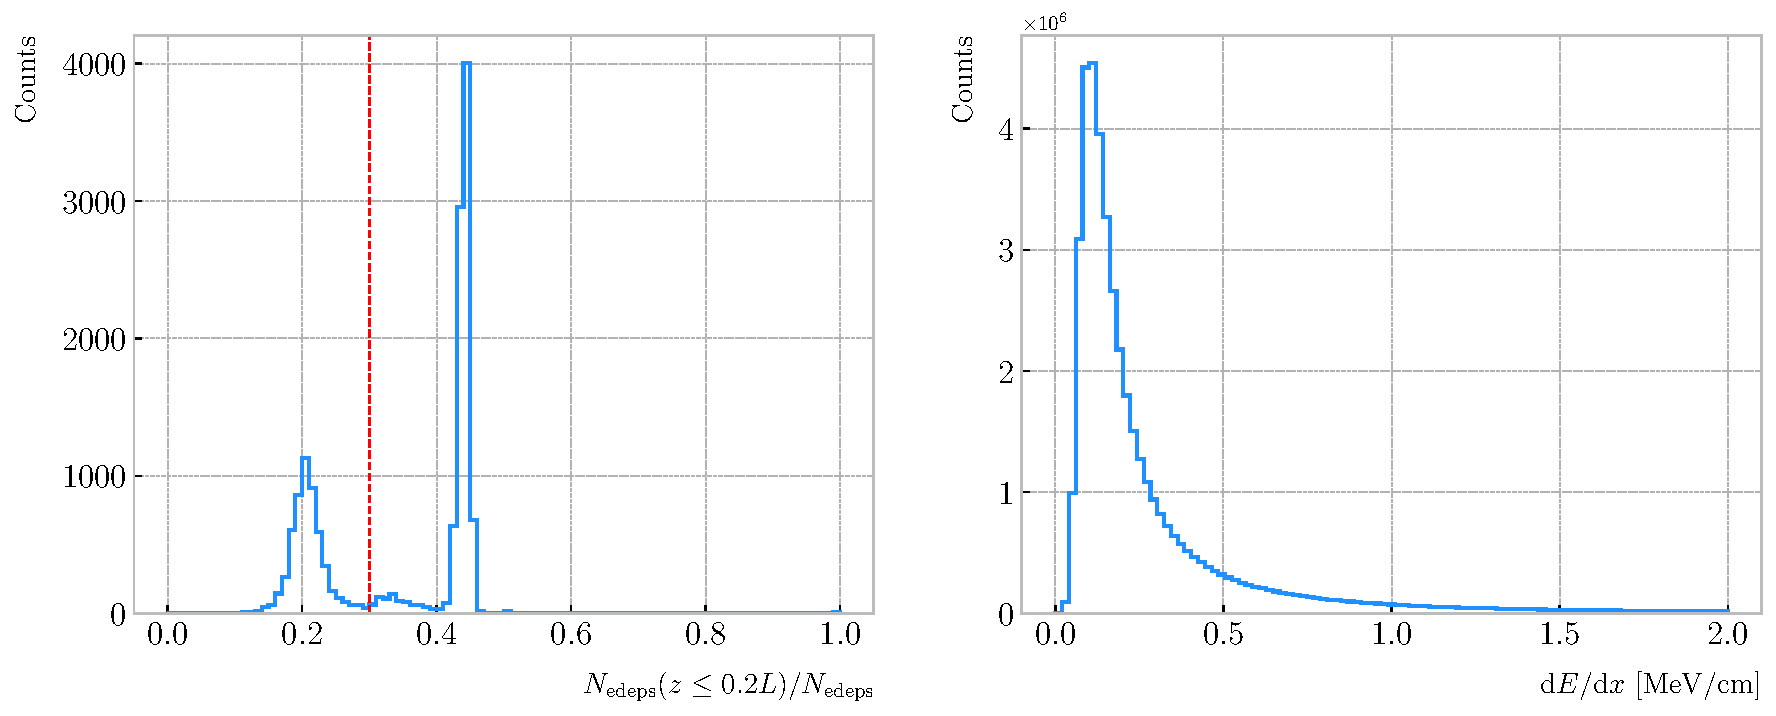
\includegraphics[width=.99\linewidth]{Images/GArSoft_PID/dEdx/geant_selection_dEdx.pdf}
	\caption[Distribution of the \texttt{Geant4}-level energy deposits per unit length in the stopping proton sample.]{Left panel: distribution of the fraction of \texttt{Geant4}-level energy deposits per track with residual range less than $20\%$ of the total track length, for the isotropic proton sample. Right panel: distribution of the ionisation per unit length of the energy deposits in the proton sample after removing the tracks with less than $30\%$ of their energy deposits in the last $20\%$ of the track.}
	\label{fig:geant_edeps}
\end{figure}

For studying the energy loss of the protons, I select the reconstructed tracks that range out (i.e. slow down to rest) inside the \gls{hpgtpc}. A characteristic feature of the energy loss profile of any stopping ionising particle is the so-called Bragg peak, a pronounced peak that occurs immediately before the particle comes to rest. From Eq. (\ref{Eq:3.1}) we can see that this behaviour is expected, as the energy loss for non-relativistic particles is inversely proportional to $\beta^{2}$. In data, a way of identifying the Bragg peak, and thus select the stopping particles, is checking the number of energy deposits towards the end of the track. In this case, I count the fraction of the \texttt{Geant4}-simulated energy deposits with a residual range value (the distance from a given energy deposit to the last deposit in the track trajectory) less than a $20\%$ of the corresponding track length\footnote{As we are applying this selection at the \texttt{Geant4}-level we could have simply selected the stopping protons using the \texttt{EndProcess} labels from the simulation. However, the Bragg peak identification method displayed here could serve as a starting point for a selection of stopping protons in real data.}. The distribution of this fraction of energy deposits for the proton sample is shown in Fig. \ref{fig:geant_edeps} (left panel). We can clearly see two well separated peaks in this distribution, one centered at $0.2$ and another, narrower one centered at a higher value. The first one corresponds to non-stopping protons, as in that case the number of energy deposits towards the end of the track is uniformly distributed due to the absence of the Bragg peak. In that way, I apply a cut in this distribution, requiring that at least $30\%$ of the simulated energy deposits sit in the last $20\%$ of the tracks, to ensure that the Bragg peak is present.

\begin{figure}[t]
	\centering
	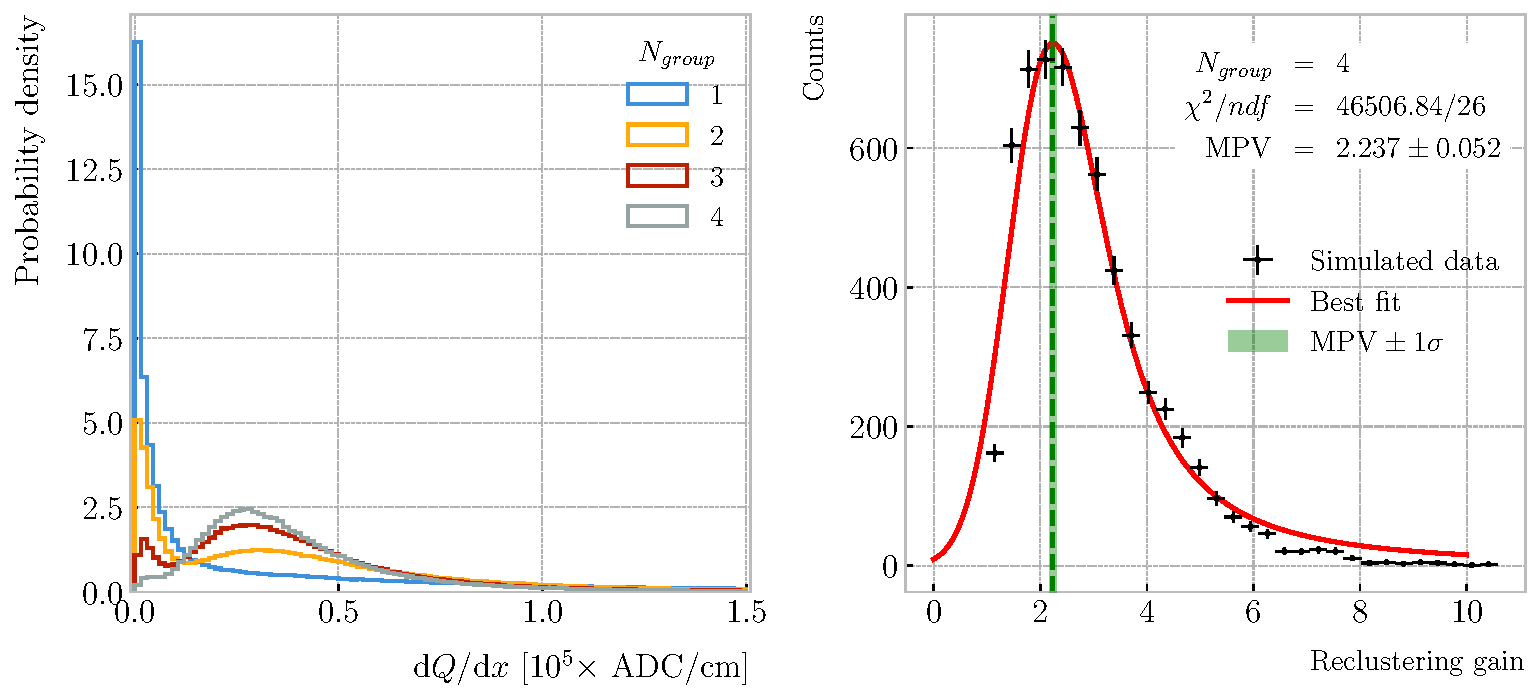
\includegraphics[width=.99\linewidth]{Images/GArSoft_PID/dEdx/reco_dQdx_groups_and_dQdx_recluster_gain.pdf}
	\caption[Distribution of the reconstructed ionisation charge per unit length for different reclustering values.]{Left panel: distribution of the reconstructed ionisation charge per unit length for our \gls{mc} stopping proton sample. The different colors indicate how many consecutive $\mathrm{d}Q/\mathrm{d}x$ pairs were grouped together. Right panel: distribution of the median change in $\mathrm{d}Q/\mathrm{d}x$ per track after $N_{group}=4$ clusters were reclustered together.}
	\label{fig:reco_dQ_groups}
\end{figure}

Figure \ref{fig:geant_edeps} (right panel) shows the distribution of the energy loss per unit length for the \texttt{Geant4}-simulated energy deposits of the selected stopping protons. We can see that it follows the expected shape of a Landau distribution, which describes the fluctuations of the ionisation energy losses \cite{Landau1944}. This distribution has a characteristic asymmetric \gls{pdf}, with a long right tail that translates into a high probability for high-energy ionisation losses. The origin of these fluctuations is mainly the possibility of transferring a high enough energy to an electron, so it becomes a ionising particle itself.

Now, from the point of view of the reconstruction, the objects that we have available to extract the ionisation information for the different reconstructed tracks are the collections of $\mathrm{d}Q$ and $\mathrm{d}x$ pairs, as stated before. The $\mathrm{d}Q$ values come from adding up the amplitude of all the reconstructed hits in a cluster, which are the input objects to the Kalman fit.

Figure \ref{fig:reco_dQ_groups} (left panel) shows the distribution of the ionisation charge deposits per unit length for the tracks in the stopping proton sample (blue line). As one may notice, this distribution does not resemble the expected shape of the Landau \gls{pdf}. This distribution peaks sharply at $0$ and has a heavy-tailed behaviour. Notice, however, how the distribution changes its shape as we group together $N_{group}$ consecutive charge deposit pairs (red, purple and green lines). The distribution in the $N_{group} = 4$ case already has a shape which resembles that of the \texttt{Geant4}-level ionisation per unit length, so I will proceed using this amount of reclustering for the reconstruction-level depositions.

An extra factor I need to account for, when reclustering is applied, is how the overall $\mathrm{d}Q/\mathrm{d}x$ per track changes. To do so, we can look at the ratio between the median $\mathrm{d}Q/\mathrm{d}x$ before and after the reclustering. Figure \ref{fig:reco_dQ_groups} (right panel) shows the median enhancement in $\mathrm{d}Q/\mathrm{d}x$ per track for the stopping proton sample in the case $N_{group}=4$. Fitting a LanGauss distribution, I estimate the most probable value of this ratio to be $G_{group} = 2.24 \pm 0.05$.

\begin{figure}[t]
	\centering
	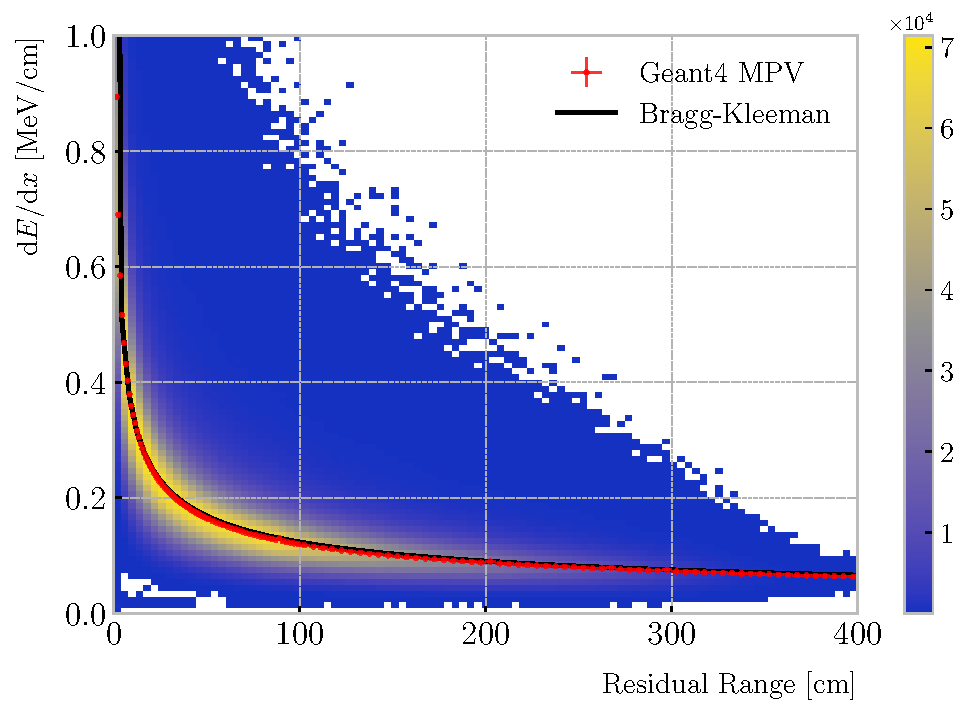
\includegraphics[width=.85\linewidth]{Images/GArSoft_PID/dEdx/bragg_kleeman_geant_langau.pdf}
	\caption[Distribution of the \texttt{Geant4}-simulated energy losses per unit length versus residual range for the stopping proton sample.]{Distribution of the \texttt{Geant4}-simulated energy losses per unit length versus residual range for the stopping proton sample. The overlaid points represent the fitted most probable value of the $\mathrm{d}E/\mathrm{d}x$ distribution in each residual range bin, whereas the curve is their best fit to the Bragg-Kleeman formula from Eq. (\ref{Eq:3.4}).}
	\label{fig:bragg_kleeman}
\end{figure}

At this point, I am left with determining the conversion between the charge deposits per unit length $\mathrm{d}Q/\mathrm{d}x$ and the energy deposits per unit length $\mathrm{d}E/\mathrm{d}x$. To this end, we need a way of comparing the two. I can use the residual range $z$ to get a prediction of the most probable $\mathrm{d}E/\mathrm{d}x$ by using the following empirical parametrisation:
\begin{equation}\label{Eq:3.4}
	\frac{\mathrm{d}E}{\mathrm{d}x}(z) = \frac{z^{\frac{1}{p}-1}}{p\Lambda^{\frac{1}{p}}},
\end{equation}
which is quoted in the literature as the Bragg-Kleeman formula \cite{Ulmer2010}. In order to obtain the $p$ and $\Lambda$ parameters I perform a fit using the energy losses and the residual ranges given by the \texttt{Geant4} stage of our proton sample.

\begin{figure}[t]
	\centering
	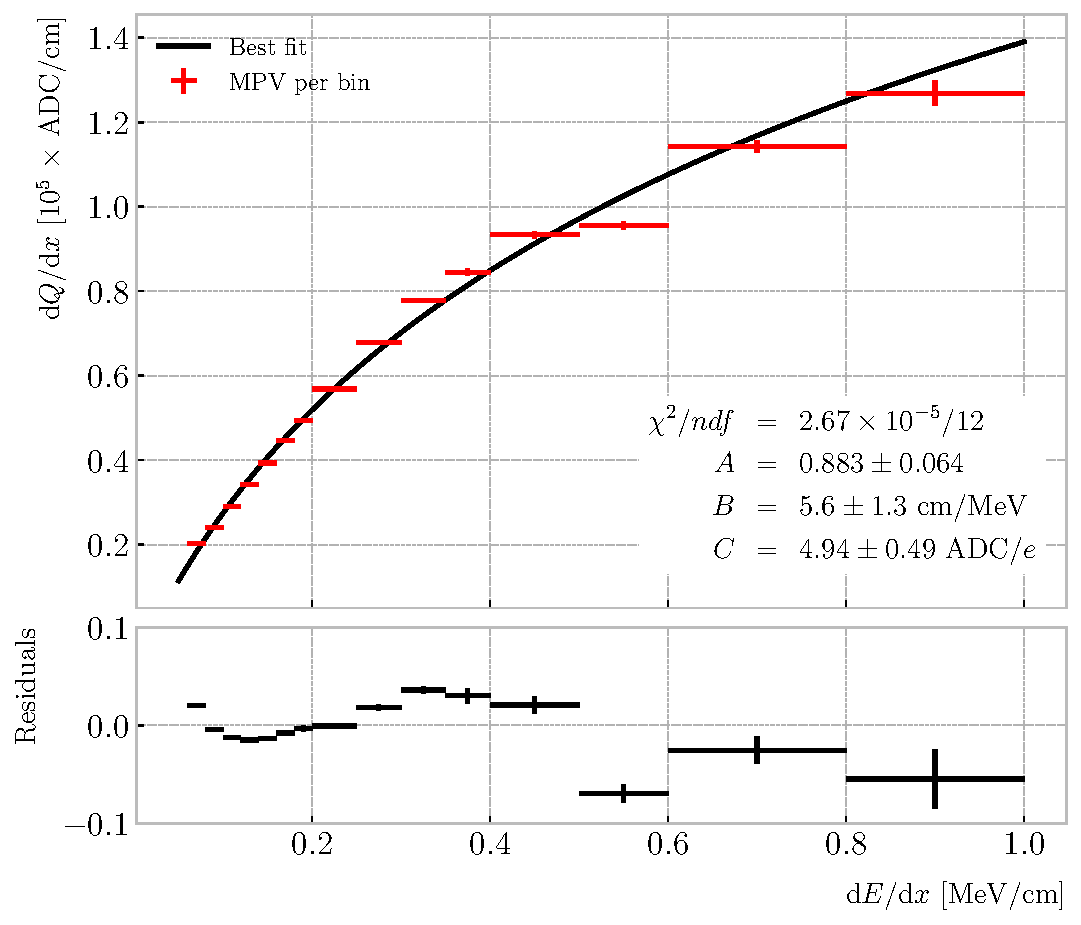
\includegraphics[width=.85\linewidth]{Images/GArSoft_PID/dEdx/dEdx_vs_dQdx_log_fit.pdf}
	\caption[Fitted most probable $\mathrm{d}Q/\mathrm{d}x$ values for each $\mathrm{d}E/\mathrm{d}x$ bin, together with best fit to the logarithmic calibration function.]{Fitted most probable $\mathrm{d}Q/\mathrm{d}x$ values for each $\mathrm{d}E/\mathrm{d}x$ bin (red points), obtained from the stopping proton sample. The overlaid curve (black line) represents the best fit to the logarithmic calibration function from Eq. (\ref{Eq:3.5}).}
	\label{fig:energy_calibration}
\end{figure}

Within our simulation, the residual range is sampled with a maximum size of $5~\mathrm{mm}$. Therefore, to perform the fit to the Bragg-Kleeman formula we can use a fine-grained residual range binning. For each of the residual range bins I extract the $\mathrm{d}E/\mathrm{d}x$ distribution and fit it to a LanGauss distribution, to obtain the value of the most probable $\mathrm{d}E/\mathrm{d}x$ in the bin together with a statistical uncertainty. I then fit Eq. (\ref{Eq:3.4}) to these most probable values and the centres of the residual range bins. This procedure is depicted in Fig. \ref{fig:bragg_kleeman}, where I show the distribution of the energy loss per unit length versus the residual range, together with the most probable $\mathrm{d}E/\mathrm{d}x$ values and their uncertainty in each bin (red points) and the curve with the best fit of the Bragg-Kleeman relation to those values (black line). The best fit is obtained for the parameter values $p = 1.8192 \pm 0.0005$ and $\Lambda = 0.3497 \pm 0.0008~\mathrm{cm}/\mathrm{MeV}^{p}$\footnote{These strange units for $\Lambda$ come from dimensional analysis, just to keep the Bragg-Kleeman formula (\ref{Eq:3.4}) consistent.}.

Having an analytical expression that relates the residual range to $\mathrm{d}E/\mathrm{d}x$, I can take our reconstruction-level residual ranges from the stopping proton sample and compute the most probable energy loss associated.

In order to parametrise the charge saturation, we can use the following logarithmic function inspired by the modified box model for recombination \cite{ArgoNeuT2013}:
\begin{equation}\label{Eq:3.5}
	\frac{\mathrm{d}E}{\mathrm{d}x} = \frac{\mathrm{e}^{\frac{\mathrm{d}Q}{\mathrm{d}x}B\frac{W_{ion}}{G_{group}C}}-A}{B},
\end{equation}
where $A$ and $B$ are the calibration parameters we need to determine, $W_{ion}$ is the average energy to produce an electron-ion pair, $G_{group}$ is the gain from the reclustering discussed above, and $C$ is the calibration constant to convert the number of electrons to \gls{adc}  counts, commonly refer to as gain (also to be obtained in the fit). In this case, I use a value for the electron-ion production energy of $W_{ion} = 26.4 \ \mathrm{eV}$ \cite{Aprile2008}. This value, used in our simulation as well, was measured for gaseous argon in normal conditions, and therefore should be checked in the future to describe correctly the high-pressure argon-$\mathrm{CH}_{4}$ mixture of \gls{ndgar}.

For the calibration fit I follow a procedure similar to the previous one for Eq. (\ref{Eq:3.4}). Binning the $\mathrm{d}E/\mathrm{d}x$ range, I fit a LanGauss function to the corresponding $\mathrm{d}Q/\mathrm{d}x$ distribution to obtain the most probable value. The resulting data points (red bars) are shown in Fig. \ref{fig:energy_calibration} (top panel), the horizontal error bars depict the width of the $\mathrm{d}E/\mathrm{d}x$ bin whereas the vertical bars represent the error associated to the most probable value estimation. A fit to the logarithmic function in Eq. (\ref{Eq:3.5}) is also shown (black line). For this I weighted the data points using the inverse of their relative error, obtaining a reduced chi-square value of $\chi^{2}/ndf=2.22\times10^{-6}$. The best fit parameters I found from this fit are $A = 0.883 \pm 0.064$, $B=5.6\pm1.3~\mathrm{cm}/\mathrm{MeV}$ and $C = 4.94 \pm 0.49 \ \mathrm{ADC}/e$. Figure \ref{fig:energy_calibration} (bottom panel) shows the residuals between the data points and the fit.

\begin{comment}
For the calibration fit I follow a procedure similar to the previous one for Eq. (\ref{Eq:3.4}). Binning the $\mathrm{d}E/\mathrm{d}x$ range, I fit a LanGauss distribution to the corresponding $\mathrm{d}Q/\mathrm{d}x$ distribution to obtain the most probable value. The resulting data points (red bars) are shown in Fig. \ref{fig:energy_calibration} (top panel), the horizontal error bars depict the width of the $\mathrm{d}E/\mathrm{d}x$ bin whereas the vertical bars represent the error associated to the most probable value estimation. Two different fits to the logarithmic function in Eq. (\ref{Eq:3.5}) are also shown. In the first case I weighted the data points using the inverse of their relative error (blue line), obtaining a reduced chi-square value of $\chi^{2}/ndf=2.22\times10^{-6}$. The best fit parameters I found from this fit are $A = 0.883 \pm 0.064$, $B=5.6\pm1.3~\mathrm{cm}/\mathrm{MeV}$ and $C = 4.94 \pm 0.49 \ \mathrm{ADC}/e$. In the second case, I performed the fit using unweighted data (yellow line). The reduced chi-square is slightly worse, with $\chi^{2}/ndf=6.95\times10^{-4}$, but the fit parameters fall in a similar range, obtaining $A = 0.76 \pm 0.10$, $B=7.8\pm1.5~\mathrm{cm}/\mathrm{MeV}$ and $C = 5.75 \pm 0.59 \ \mathrm{ADC}/e$. Figure \ref{fig:energy_calibration} (bottom panel) shows the (unweighted) residuals between the data points and the two fits. It can be seen that both fits behave similarly in the low ionisation loss regime, but the unweighted fit manages to capture the behaviour at high energies better.
\end{comment}

\begin{comment}
\begin{table}
	\caption{Calibration parameters obtained from the fit of the \gls{ndgar} simulated stopping proton sample to the calibration function from Eq. (\ref{Eq:3.5}). The fits were performed for the 10, 12, and 16-bit \gls{adc}  limits and using weighted and unweighted data points, as described in the text.}
	\begin{center}
		\begin{small}
			\begin{tabular}{llllll}
				\cline{3-6}
				\multicolumn{2}{l}{\multirow{2}{*}{}}                                          & \multirow{2}{*}{$\chi^{2}/ndf$} & \multicolumn{3}{l}{Best fit $\pm 1\sigma$}                              \\ \cline{4-6} 
				\multicolumn{2}{l}{}                                                           &                                 & $A$             & $B~(\mathrm{cm}/\mathrm{MeV})$ & $C~(\mathrm{ADC}/e)$ \\ \hline
				\multicolumn{1}{l|}{\multirow{2}{*}{10-bit}} & \multicolumn{1}{l|}{Weighted}   & $1.83\times10^{-6}/12$          & $-9.3\pm3.9$    & $270\pm69$                     & $27.1\pm5.4$         \\
				\multicolumn{1}{l|}{}                        & \multicolumn{1}{l|}{Unweighted} & $2.32\times10^{-3}/12$          & $0.0\pm2.2$     & $86\pm45$                      & $11.4\pm4.5$         \\ \hline
				\multicolumn{1}{l|}{\multirow{2}{*}{12-bit}} & \multicolumn{1}{l|}{Weighted}   & $2.67\times10^{-5}/12$          & $0.883\pm0.064$ & $5.6\pm1.3$                    & $4.94\pm0.49$        \\
				\multicolumn{1}{l|}{}                        & \multicolumn{1}{l|}{Unweighted} & $8.35\times10^{-3}/12$          & $0.76\pm0.10$   & $7.8\pm1.5$                    & $5.75\pm0.59$        \\ \hline
				\multicolumn{1}{l|}{\multirow{2}{*}{16-bit}} & \multicolumn{1}{l|}{Weighted}   & $1.44\times10^{-5}/12$          & $0.949\pm0.024$ & $3.53\pm0.58$                  & $4.52\pm0.29$        \\
				\multicolumn{1}{l|}{}                        & \multicolumn{1}{l|}{Unweighted} & $5.71\times10^{-3}/12$          & $0.850\pm0.054$ & $5.59\pm0.79$                  & $5.43\pm0.39$        \\ \hline
			\end{tabular}
		\end{small}
	\end{center}
	\label{tab:calibration_fits}
\end{table}
\end{comment}

The value for the gain I obtained from the fit is in reasonable agreement with our expectation. This value is set in GArSoft to $5 \ \mathrm{ADC}/e$ by default.

\begin{comment}
\begin{table}[h!]
	\caption{Effective recombination parameters obtained from the fit of \gls{ndgar} simulated stopping proton sample to the modified box model. The corresponding parameters obtained by the LAr \gls{tpc} experiments ArgoNeuT, $\mu$BooNE and ProtoDUNE are also shown for comparison.}
	\begin{center}
		\begin{tabular}{lcccc}
			\hline
																						   & ArgoNeuT        & $\mu$BooNE     & ProtoDUNE  & \gls{ndgar} \\ \hline
			modified box model $\alpha$                                                    & $0.93\pm0.02$   & $0.92\pm0.02$  & $0.93\pm0.02$ & $0.91\pm0.02$       \\ \hline
			modified box model $\beta'$\\ $(\mathrm{kV/cm})(\mathrm{g/cm^{2}})/\mathrm{MeV}$ & $0.212\pm0.002$ & $0.184\pm0.02$ & $0.20\pm0.03$ & $0.040\pm0.004$     \\ \hline
			\end{tabular}
	\end{center}
	\label{tab:modified_box_fits}
\end{table}
\end{comment}

\begin{figure}[t]
	\centering
	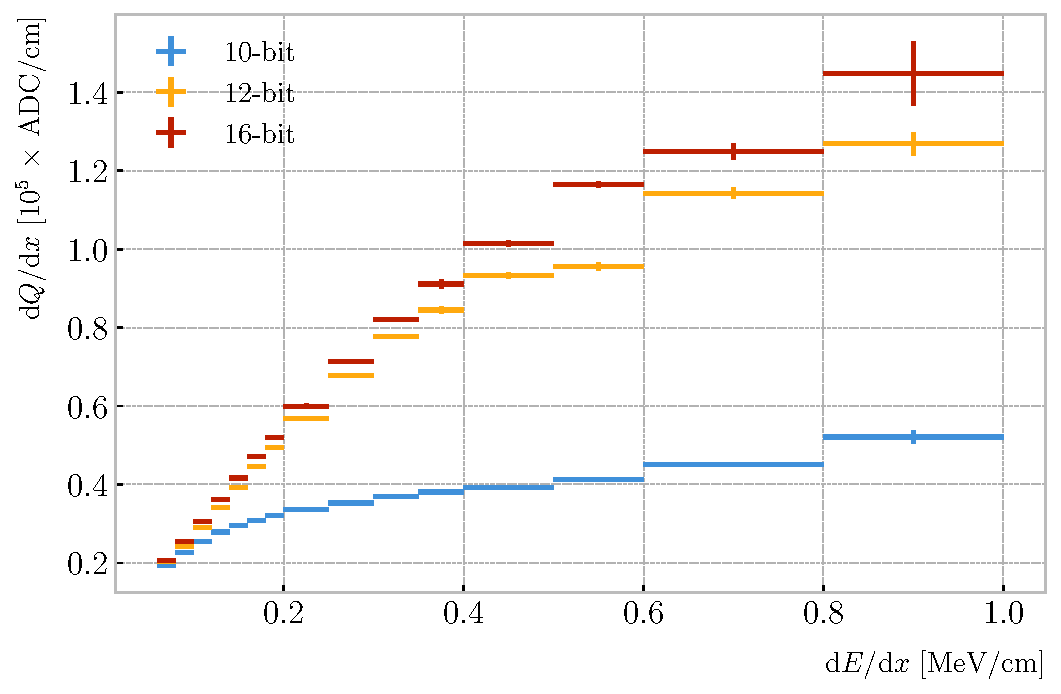
\includegraphics[width=.85\linewidth]{Images/GArSoft_PID/dEdx/dEdx_vs_dQdx_ADC_saturation_mpv.pdf}
	\caption[Fitted most probable $\mathrm{d}Q/\mathrm{d}x$ values for each $\mathrm{d}E/\mathrm{d}x$ bin for three different \gls{adc}  bit limits.]{Fitted most probable $\mathrm{d}Q/\mathrm{d}x$ values for each $\mathrm{d}E/\mathrm{d}x$ bin for three different \gls{adc}  bit limits, 10 (blue points), 12 (default, yellow points) and 16-bit (red points).}
	\label{fig:energy_adc_saturation}
\end{figure}

\begin{table}[t]
	\caption[Calibration parameters obtained from the fit of the \gls{ndgar} simulated stopping proton sample to the calibration function.]{Calibration parameters obtained from the fit of the \gls{ndgar} simulated stopping proton sample to the calibration function from Eq. (\ref{Eq:3.5}). The fits were performed for the 10, 12, and 16-bit \gls{adc}  limits.}
	\begin{center}
		\begin{small}
			\begin{tabular}{cc|ccc}
				\multirow{2}{*}{}           &                            & \multicolumn{3}{c}{Best fit $\pm ~ 1\sigma$}                              \\[2mm] \cline{3-5} 
											& $\chi^{2}/ndf$             & \rule{0pt}{1.1\normalbaselineskip}$A$               & $B~(\mathrm{cm}/\mathrm{MeV})$ & $C~(\mathrm{ADC}/e)$ \\[2mm] \hline
				\multicolumn{1}{c|}{\rule{0pt}{1.1\normalbaselineskip}10-bit} & $1.83 \times 10^{-6} / 12$ & $-9.3 \pm 3.9$    & $270 \pm 69$                   & $27.1 \pm 5.4$       \\[2mm]
				\multicolumn{1}{c|}{12-bit} & $2.67 \times 10^{-5} / 12$ & $0.883 \pm 0.064$ & $5.6 \pm 1.3$                  & $4.94 \pm 0.49$      \\[2mm]
				\multicolumn{1}{c|}{16-bit} & $1.44 \times 10^{-5} / 12$ & $0.949 \pm 0.024$ & $3.53 \pm 0.58$                & $4.52 \pm 0.29$     
			\end{tabular}
		\end{small}
	\end{center}
	\label{tab:calibration_fits}
\end{table}

One interesting thing to check is what induces this non-linear relation between charge and energy. The only effects that modify the amount of electrons reaching the readout planes in the simulation are the transverse diffusion and the finite electron lifetime. Once the electrons reach the readout chambers, the pad response functions are applied, together with an electrons-to-\gls{adc}  conversion and the \gls{adc}  saturation limit.

\begin{figure}[t]
	\centering
	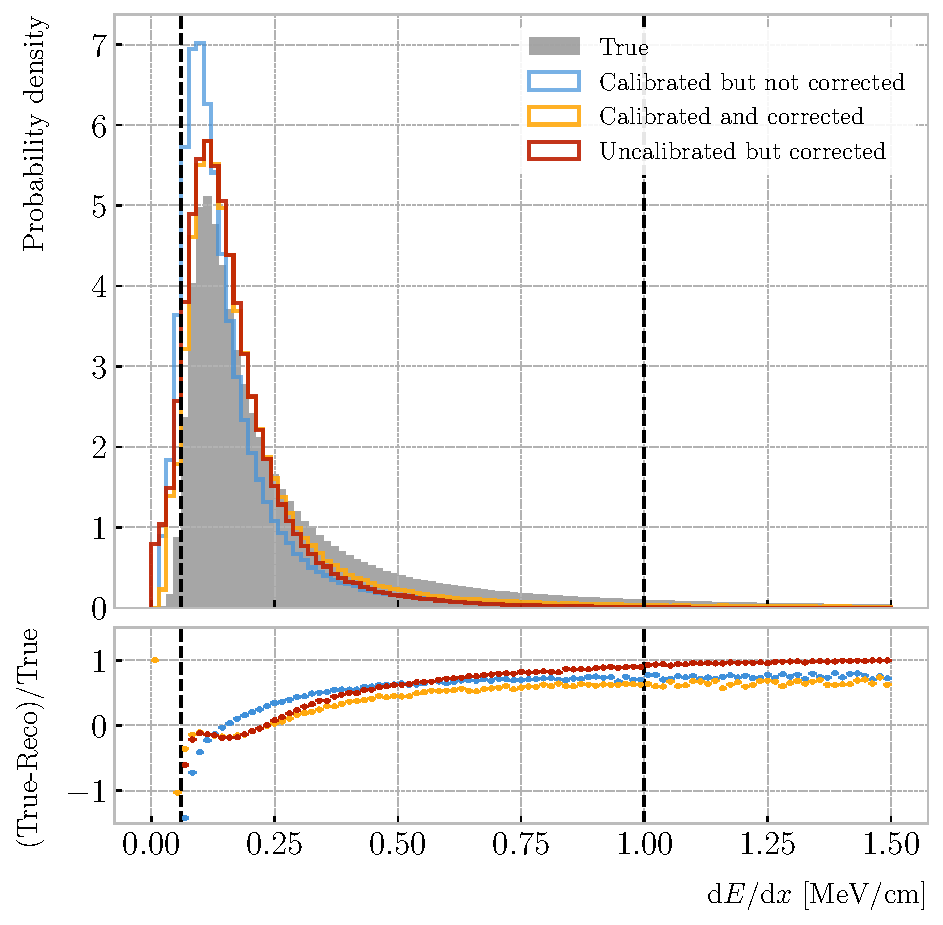
\includegraphics[width=.80\linewidth]{Images/GArSoft_PID/dEdx/reco_dEdx_corrected_1d.pdf}
	\caption[Area normalised $\mathrm{d}E/\mathrm{d}x$ distributions for the true and the reconstructed energy deposits in the stopping proton sample.]{Top panel: area normalised $\mathrm{d}E/\mathrm{d}x$ distributions for the true (solid grey) and the reconstructed energy deposits in the stopping proton sample, both after applying the calibration (blue) and the calibration and the normalisation correction (yellow). Also shown is the distribution obtained by applying a correction factor to the $\mathrm{d}Q/\mathrm{d}x$ values but not the calibration (red). Bottom panel: fractional residuals for the uncorrected (blue), corrected (yellow) and uncalibrated (red) samples.}
	\label{fig:energy_correction}
\end{figure}

By default, GArSot applies a 12-bit \gls{adc}  limit, which can be changed in the simulation configuration. However, it can only be increased up to 16-bit, as we represent the \gls{adc}  collection as a \texttt{std::vector<short>}. This way, I tried to change the saturation parameter to see how it affects the relation between reconstructed charge and energy. Figure \ref{fig:energy_adc_saturation} shows a comparison between the most probable $\mathrm{d}Q/\mathrm{d}x$ for 10, 12 and 16-bit \gls{adc}  limits. As expected, the lower the limit is the sooner the charge saturates. For higher \gls{adc}  limits the relation between energy and charge remains linear up to higher $\mathrm{d}E/\mathrm{d}x$ values, but even for the 16-bit limit the saturation is noticeable for ionisations $\geq 0.5 ~ \mathrm{MeV}/\mathrm{cm}$.

Table \ref{tab:calibration_fits} shows the results of fitting the samples with 10, 12, and 16-bits \gls{adc}  limits to the calibration function from Eq. (\ref{Eq:3.5}), using the weights based on their relative error as described previously. One interesting feature to notice is how different the best fit parameters look for the 10-bit \gls{adc}  saturation when compared to the other two, which are consistent with each other.

At this point we can compare the $\mathrm{d}E/\mathrm{d}x$ distribution one gets from \texttt{Geant4}, i.e. the true energy loss distribution, and the distribution I found by applying the calibration function to our collection of reconstructed $\mathrm{d}Q/\mathrm{d}x$ values. Figure \ref{fig:energy_correction} (top panel) shows the true (solid grey) and reconstructed (blue) distributions together. The dashed vertical lines indicate the region of validity of the calibration fit, i.e. the left and right edges of the first and last $\mathrm{d}E/\mathrm{d}x$ bins, respectively. Notice that these histograms are area-normalised, as the total number of true energy deposits is much higher than the number of reconstructed charge deposits. This is due to a combination of effects, like the finite spatial resolution of the detector, the hit clustering used in the track fitting and the reclustering we have applied here.

The two distributions are significantly different. That can be seen clearly when looking at the fractional residuals, shown in Fig. \ref{fig:energy_correction} (bottom panel). In particular, the position of the peak is off, which could bias the mean energy loss predictions. It seems like the difference between these may be due to an overall scaling factor. One possibility is to scale the most probable value of the reconstructed distribution to the most probable value predicted by \texttt{Geant4}. I do this by fitting both distributions using a LanGauss function, obtaining $\mathrm{d}E/\mathrm{d}x_{\mathrm{MPV}, ~true} = 0.1145\pm0.0005~\mathrm{MeV}/\mathrm{cm}$ and $\mathrm{d}E/\mathrm{d}x_{\mathrm{MPV}, ~reco} = 0.0928\pm0.0005~\mathrm{MeV}/\mathrm{cm}$ for the true and reconstructed most probable values, respectively. These can be translated into an scaling factor $S=0.579\pm0.006$.

The result of applying the scaling correction can be seen in Fig. \ref{fig:energy_correction} (top panel). The calibrated and corrected $\mathrm{d}E/\mathrm{d}x$ distribution (yellow) peaks around the same value the true distribution does, as expected. Moreover, the high energy region is also slightly better described. For low ionisations, below the lower limit of the calibration fit, the differences between true and reconstructed are still significant. This low energy excess may be a migration of some events from the peak region. The overall effect of the correction can be seen in the fractional residual plot in Fig. \ref{fig:energy_correction} (bottom panel).

One can also check what happens if instead of applying the logarithmic calibration we simply scale the $\mathrm{d}Q/\mathrm{d}x$ distribution (after reclustering) to have the same most probable value as the true  $\mathrm{d}E/\mathrm{d}x$ distribution. In this case, following an analogous procedure to the one described earlier, I found the scaling factor $S_{uncalibrated}=0.414\pm0.002~\mathrm{MeV}/\mathrm{ADC}$\footnote{Notice that now the scaling factor is not dimensionless, as it acts like a conversion factor here.}. The resulting uncalibrated but corrected distribution (red) is also shown in in Fig. \ref{fig:energy_correction} (top panel). The behaviour of the new distribution is similar to the corrected case at low energy losses, around the peak of the true distribution, but it is worse at describing the high energy tail. This is expected, as it is in the high ionisation regime where saturation effects apply and therefore calibration is needed.

\section{Charged pion decay in flight}
\label{section:pi_decay}

As discussed previously, in GArSoft the \gls{hpgtpc} tracks are formed after a pattern recognition algorithm and a Kalman filter are applied to the \gls{tpc} clusters. These two steps can find discontinuities in the track candidates (e.g. due to a particle decay) when these so-called breakpoints are large enough. However, for some, more subtle, cases they may miss them and form a single reconstructed track. It has been noted in the literature that Kalman filters offer, as a by-product, additional information to form test statistics to identify these breakpoints \cite{Fruehwirth1988, Astier2000}.

\begin{figure}[t]
	\begin{subfigure}{0.5\textwidth}
		\centering
		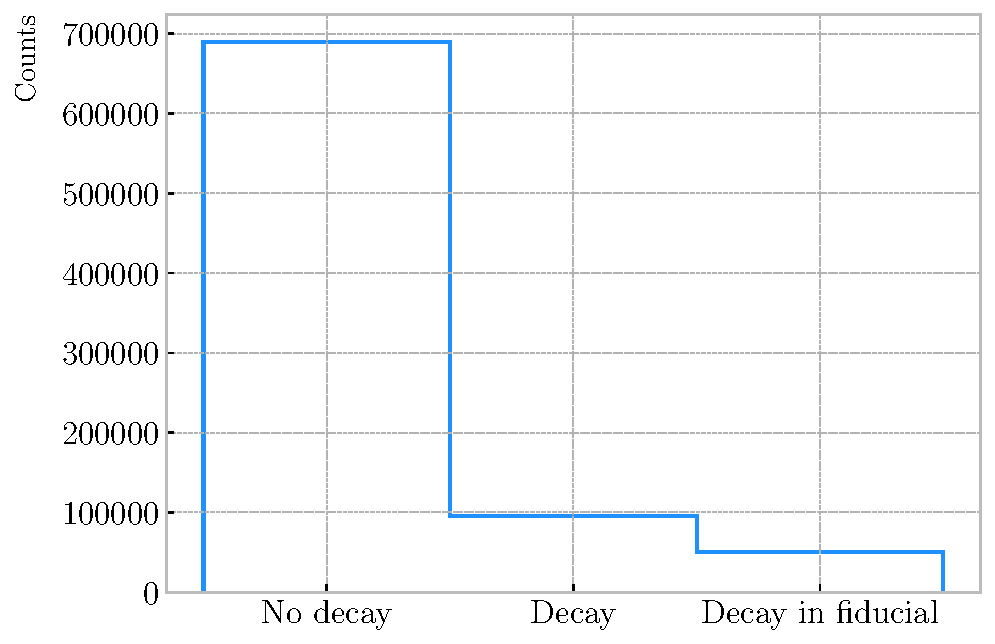
\includegraphics[width=.99\linewidth]{Images/GArSoft_PID/pion_decay/pion_decay_status.pdf}
	\end{subfigure}
	\begin{subfigure}{0.5\textwidth}
		\centering
		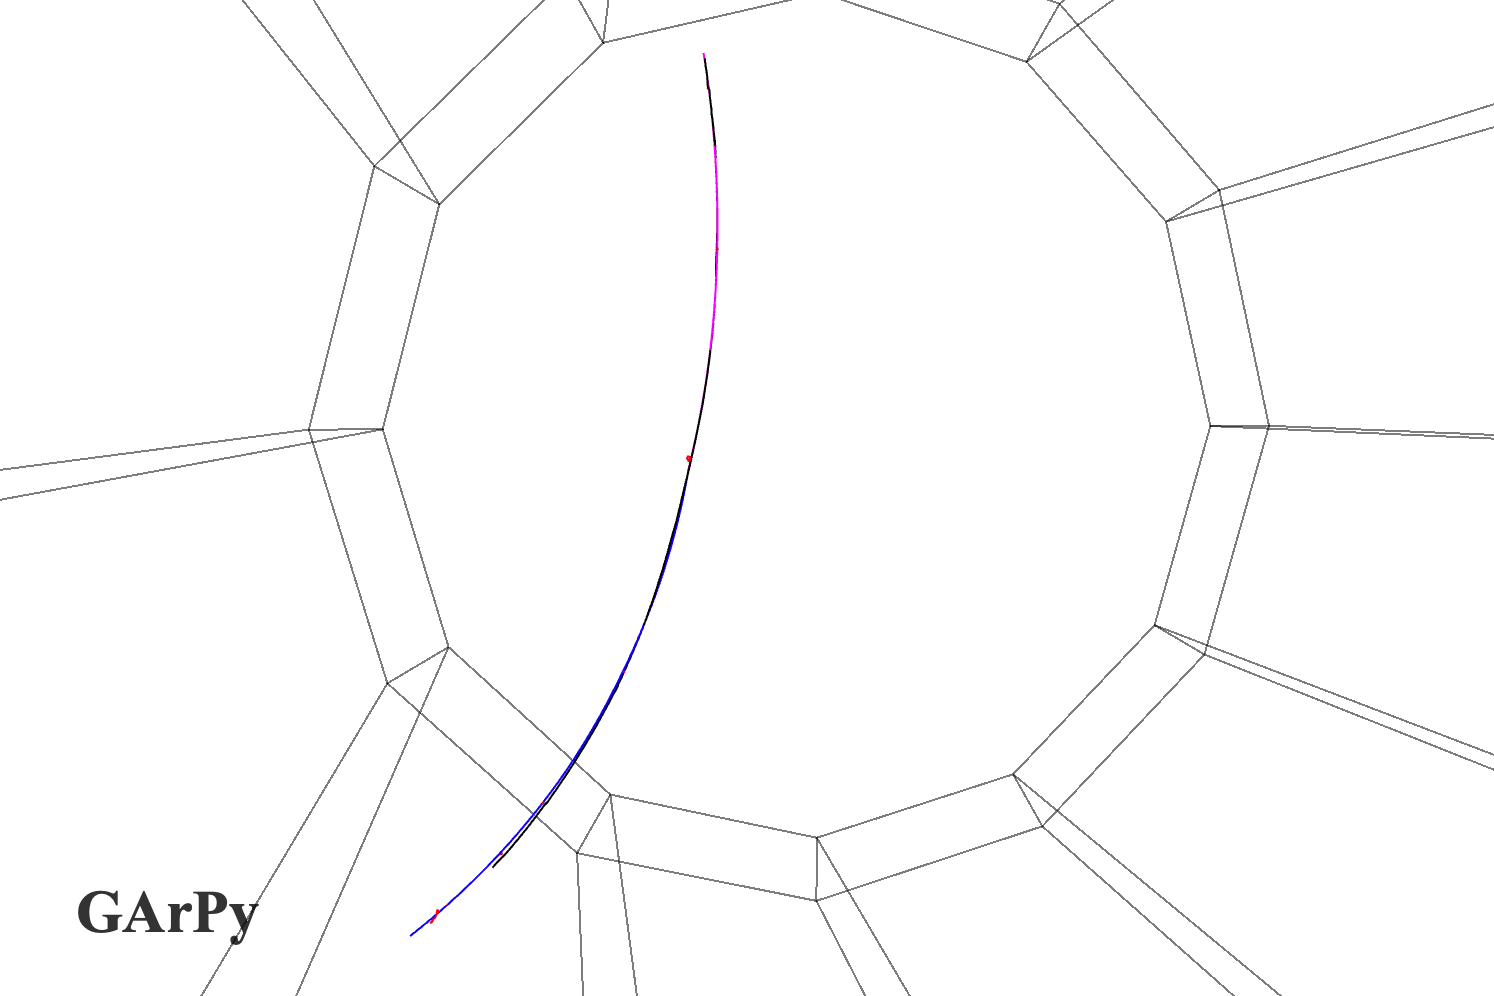
\includegraphics[width=.99\linewidth]{Images/GArSoft_PID/pion_decay/pion_decay_evd.png}
	\end{subfigure}
	\caption[Fraction of charged pions with $p=500 \ \mathrm{MeV}/c$ decaying in the \gls{hpgtpc} and example event display.]{Left panel: number of non-decaying, decaying and decaying in the fiducial volume pions for a \gls{mc} sample of $10^{5}$, $p=500 \ \mathrm{MeV}/c$ isotropic positively charged pions inside the \gls{tpc}. Right panel: event display for a positive pion decaying inside the fiducial volume, with a single reconstructed track for the pion and muon system.}
	\label{fig:pion_decays}
\end{figure}

Considering the mean life of the charged pion, $\tau = (2.6033\pm0.0005)\times10^{-8} \ \mathrm{s}$, one can estimate that about $12\%$ of the pions with momentum $p \sim \mathcal{O}(500 \ \mathrm{MeV}/c)$ (roughly the peak of the pion momentum distribution in $\nu_{\mu}$ \gls{cc} interactions off argon) decay inside the \gls{tpc}. Figure \ref{fig:pion_decays} (left panel) shows the amount of charged pions decaying in the full and fiducial \gls{hpgtpc} volumes from an isotropic, monoenergetic sample of $10^{5}$ negatively charged pions with $p=500 \ \mathrm{MeV}/c$. We see that about $10\%$ of those decayed, with more than half of them decaying inside the \gls{tpc} fiducial volume.

Figure \ref{fig:pion_decays} (right panel) shows an example event display of a charged pion (magenta line) which decays in flight inside the \gls{tpc}. However, because the angle of the muon (blue line) is small both were reconstructed as one single track (black line). In this case, the composite track reaches the \gls{ecal}, where it undergoes a muon-like interaction, thus being classified as a muon.

A way to understand what decaying pion tracks were totally or partially reconstructed together with the daughter muon is looking at the relative energy contributions to the reconstructed track. In order to select a sample of such events, I require that a minimum $50\%$ of the total energy comes from the pion and at least $20\%$ from the muon.

\subsection{Track breakpoints}

To identify potential decays we can use the information we obtain from the Kalman filter at each step of the fitted track. The simplest test we can think about is computing the $\chi^{2}$ of the mismatch between all the parameters in the forward and the backward fits:
\begin{equation}
	\chi^{2 \ (FB)}_{k} = (\hat{\mathrm{x}}^{B}_{k}-\hat{\mathrm{x}}^{F}_{k})^{T}[V^{(\hat{\mathrm{x}}_{k},B)}+V^{(\hat{\mathrm{x}}_{k},F)}]^{-1}(\hat{\mathrm{x}}^{B}_{k}-\hat{\mathrm{x}}^{F}_{k}),
\end{equation}
where $\hat{\mathrm{x}}^{F}_{k}$, $\hat{\mathrm{x}}^{B}_{k}$ are the Kalman filter state vector estimates at step $k$ in the forward and backward fits, and $V^{(\hat{\mathrm{x}}_{k},F)}$, $V^{(\hat{\mathrm{x}}_{k},B)}$ the covariance matrices of $\hat{\mathrm{x}}^{F}_{k}$ and $\hat{\mathrm{x}}^{B}_{k}$, respectively. Using the values of the $\chi^{2}$ at measurement $k$ for the forward and backward fits we can compute another $\chi^{2}$ value that characterises the overall track fit:
\begin{equation}
	\chi^{2}_{track} = \chi^{2 \ (F)}_{k} + \chi^{2 \ (B)}_{k} + \chi^{2 \ (FB)}_{k},
\end{equation}
which remains approximately constant for all $k$.

An alternative approach proposed in the context of the \gls{nomad} experiment was using a fit with a more elaborated breakpoint hypothesis, so we can perform a comparison of the $\chi^{2}$ with and without breakpoints. This can be achieved by using an alternative parametrisation, which allows some of the track parameters to be discontinuous at certain points. A decay changes the momentum magnitude and direction, so we can use the new state vector:
\begin{equation}
	\alpha=\begin{pmatrix}y,& z,& 1/R_{F},& 1/R_{B},& \phi_{F},& \phi_{B},& \mathrm{tan}\lambda_{F},& \mathrm{tan}\lambda_{B}\end{pmatrix}^{T}.
\end{equation}

\begin{figure}[t]
	\centering
	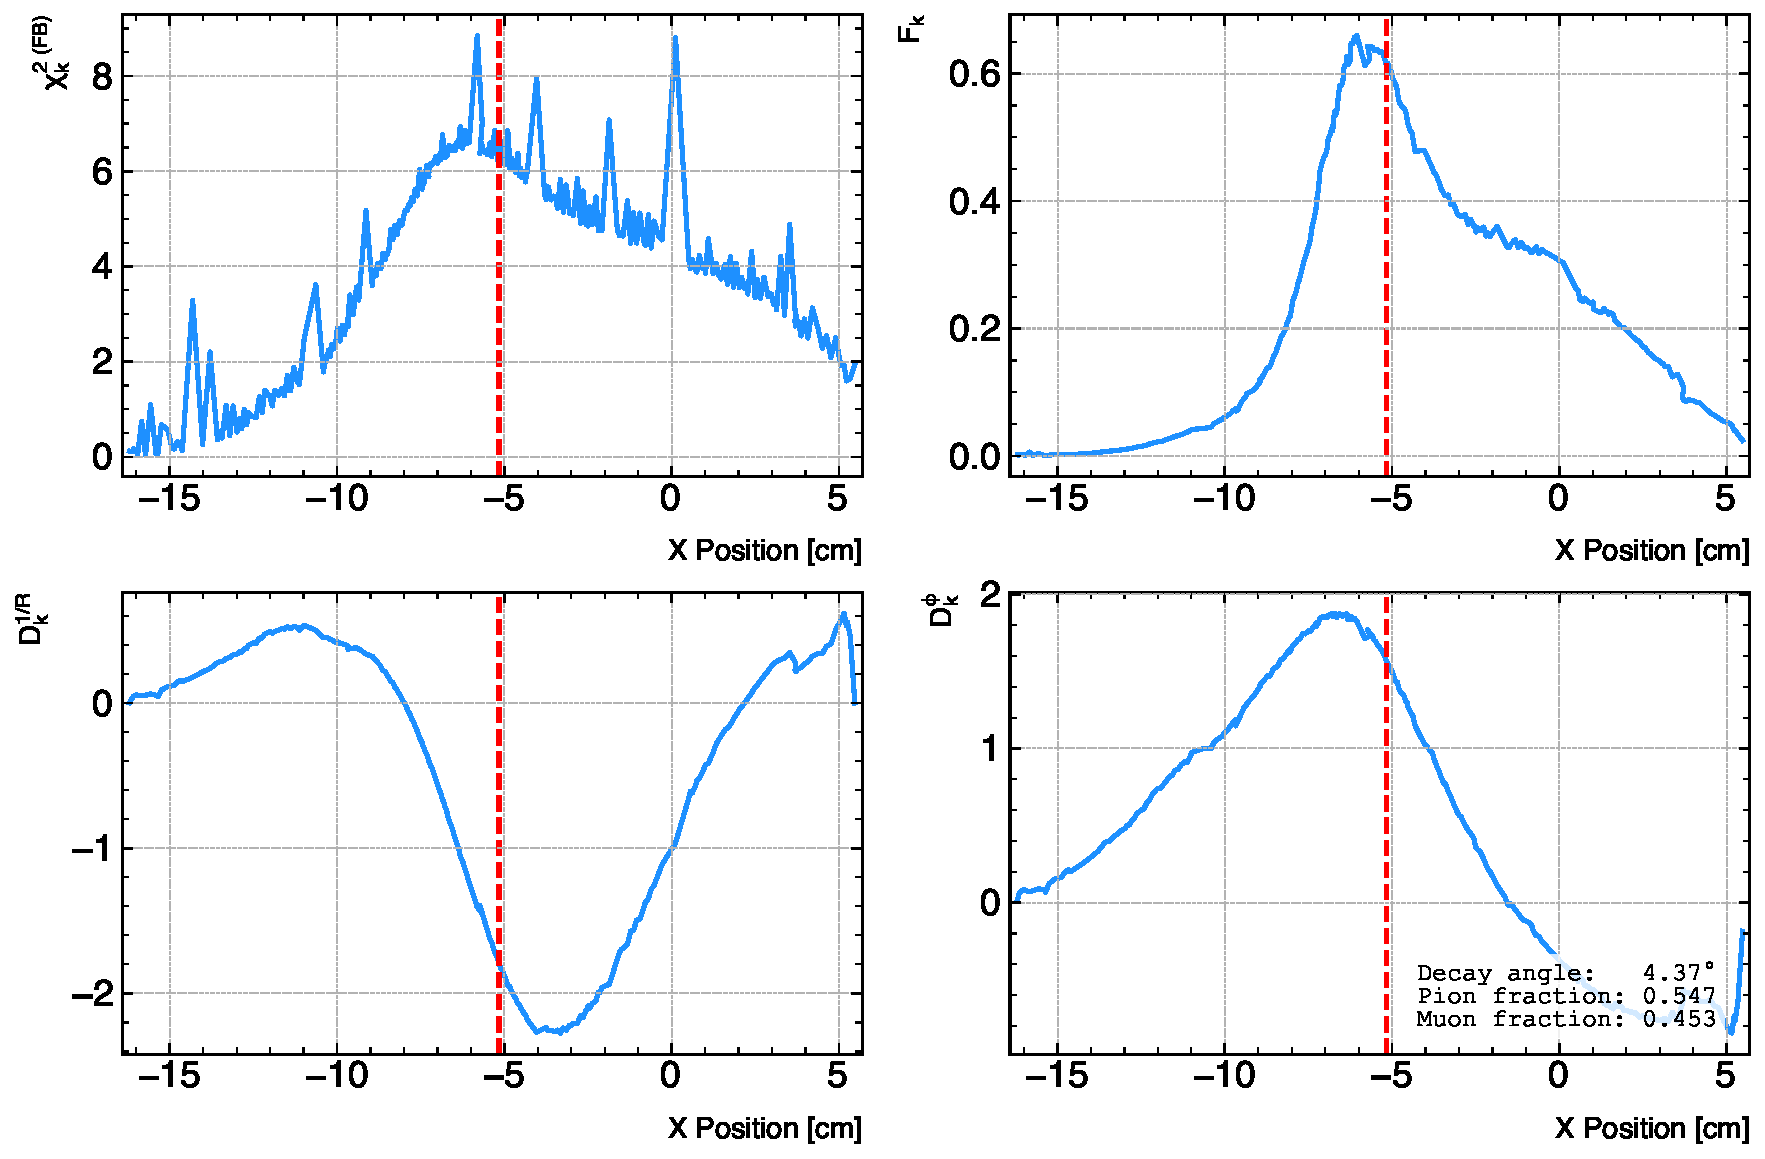
\includegraphics[width=.85\linewidth]{Images/GArSoft_PID/pion_decay/pion_decay_variables_event_425.pdf}
	\caption[Values of $\chi^{2 \ (FB)}_{k}$, $F_{k}$, $D^{1/R}_{k}$, and $D^{\phi}_{k}$ versus position along the drift direction for a reconstructed track in a $\pi^{+}$ decay event.]{Values of $\chi^{2 \ (FB)}_{k}$ (top left panel), $F_{k}$ (top right panel), $D^{1/R}_{k}$ (bottom left panel) and $D^{\phi}_{k}$ (bottom right panel) versus position along the drift direction for a reconstructed track in a positive pion decay event. The vertical red dashed line indicates the true location of the decay point.}
	\label{fig:breakpoint_variables_example}
\end{figure}

As we already have the estimates from the standard Kalman filter and their covariance matrices at each point, we do not need to repeat the Kalman fit for the new parametrisation. Instead, I can compute the values of $\alpha$ at each point $k$ that minimise the $\chi^{2}$ resulting from comparing them to $\{\hat{\mathrm{x}}^{B}_{k}, \hat{\mathrm{x}}^{F}_{k}\}$. Introducing the two $5 \times 8$ matrices:
\begin{equation}
	H^{F}=\begin{pmatrix}1&0&0&0&0&0&0&0 \\ 0&1&0&0&0&0&0&0 \\ 0&0&1&0&0&0&0&0 \\ 0&0&0&0&1&0&0&0 \\ 0&0&0&0&0&0&1&0\end{pmatrix}, \
	H^{B}=\begin{pmatrix}1&0&0&0&0&0&0&0 \\ 0&1&0&0&0&0&0&0 \\ 0&0&0&1&0&0&0&0 \\ 0&0&0&0&0&1&0&0 \\ 0&0&0&0&0&0&0&1\end{pmatrix},
\end{equation}
we can write this as:
\begin{equation}
	\begin{split}
		\chi_{k}^{2 \ (FB)} (\alpha) &= (\hat{\mathrm{x}}_{k}^{F}-H^{F}\alpha)^{T}\left[V^{(\hat{\mathrm{x}}_{k},F)}\right]^{-1}(\hat{\mathrm{x}}_{k}^{F}-H^{F}\alpha)\\
		&+(\hat{\mathrm{x}}_{k}^{B}-H^{B}\alpha)^{T}\left[V^{(\hat{\mathrm{x}}_{k},B)}\right]^{-1}(\hat{\mathrm{x}}_{k}^{B}-H^{B}\alpha).
	\end{split}
\end{equation}

The minimum of $\chi_{k}^{2 \ (FB)} (\alpha)$ is found when the measured new state vector takes the value:
\begin{equation}
	\hat{\alpha}_{k} = V^{(\hat{\alpha}_{k})} H^{T} (V^{(\hat{\mathrm{x}}_{k})})^{-1} \hat{\mathrm{X}},
\end{equation}
where $\hat{\mathrm{X}} = \{\hat{\mathrm{x}}^{B}_{k}, \hat{\mathrm{x}}^{F}_{k}\}$, $V^{(\hat{\mathrm{x}}_{k})}$ is the block diagonal matrix formed by $V^{(\hat{\mathrm{x}}_{k},F)}$ and $V^{(\hat{\mathrm{x}}_{k},B)}$ and $V^{(\hat{\alpha}_{k})}$ is the covariance matrix of $\hat{\alpha}_{k}$, given by:
\begin{equation}
	V^{(\hat{\alpha}_{k})} = \left(H^{T} (V^{(\hat{\mathrm{x}}_{k})})^{-1} H\right)^{-1}.
\end{equation}

\begin{figure}[t]
	\begin{subfigure}{0.5\textwidth}
		\centering
		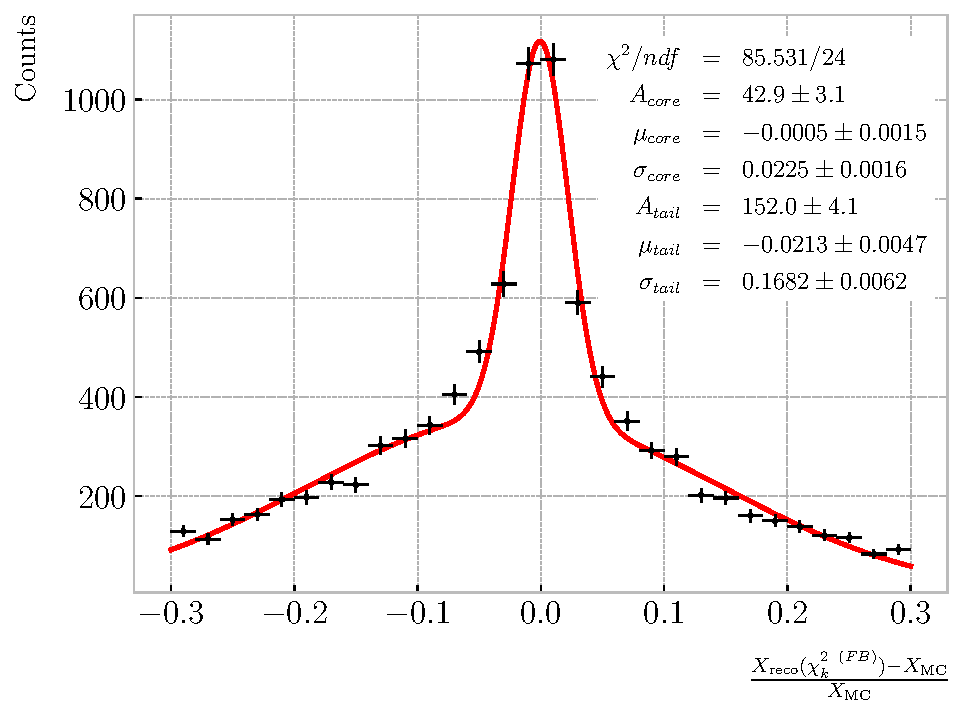
\includegraphics[width=.99\linewidth]{Images/GArSoft_PID/pion_decay/pion_decay_resolution_chisqfb.pdf}
	\end{subfigure}
	\begin{subfigure}{0.5\textwidth}
		\centering
		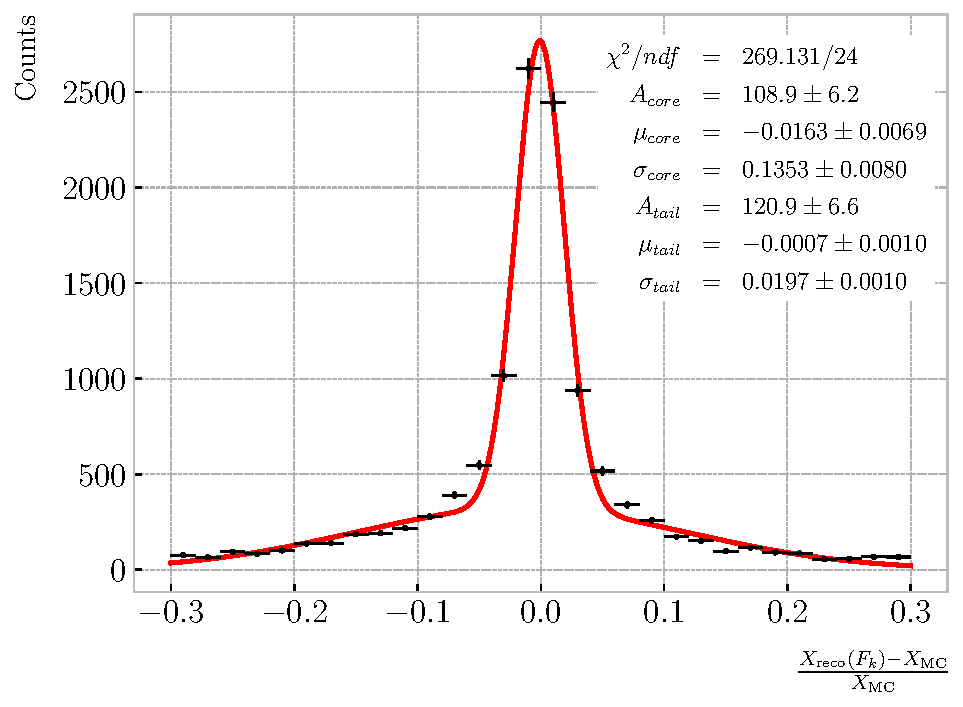
\includegraphics[width=.99\linewidth]{Images/GArSoft_PID/pion_decay/pion_decay_resolution_fisher.pdf}
	\end{subfigure}
	\caption[Residual distributions of the true and reconstructed decay position along the drift coordinate, using the position of the maximum of $\chi^{2 \ (FB)}_{k}$ and $F_{k}$ as estimates of the decay position.]{Fractional residual distributions of the true and reconstructed decay position along the drift coordinate, using the position of the maximum of $\chi^{2 \ (FB)}_{k}$ (left panel) and $F_{k}$ (right panel) as estimates of the decay position. Also shown are double Gaussian fits to these points (red lines).}
	\label{fig:pion_decay_resolution}
\end{figure}

From these new fit estimates we can compute the $F$ statistic, which tells us whether the model with breakpoint provides a statistically significant better fit:
\begin{equation}
	F_{k}=\left(\frac{\chi^{2}_{track,k}-\chi^{2}_{full,k}}{8-5}\right)/\left(\frac{\chi^{2}_{full,k}}{N-8}\right).
\end{equation}

One can also compute the signed difference of the duplicated variables divided by their standard deviation at each point. These represent how significant the discontinuity in each variable is. For any variable $\eta$ we can write it as:
\begin{equation}
	D^{\eta}_{k} = \frac{\hat{\eta}^{B}_{k}-\hat{\eta}^{F}_{k}}{\sqrt{\mathrm{Var}[\hat{\eta}^{F}_{k}]+\mathrm{Var}[\hat{\eta}^{B}_{k}]-2\mathrm{Cov}[\hat{\eta}^{F}_{k}, \hat{\eta}^{B}_{k}]}}.
\end{equation}
In our case, the relevant ones to look at are $D^{1/R}_{k}$ and $D^{\phi}_{k}$.

Figure \ref{fig:breakpoint_variables_example} shows the values of $\chi^{2 \ (FB)}_{k}$, $F_{k}$, $D^{1/R}_{k}$ and $D^{\phi}_{k}$ as functions of the position along the drift direction, for an example reconstructed track with $55.5\%$ of the energy coming from the charged pion and $45.5\%$ from the daughter muon. The true position of the decay is indicated (dashed red lines). Notice how $\chi^{2 \ (FB)}_{k}$ and $F_{k}$, $D^{1/R}_{k}$ reach their maxima near the decay point. In the former case this indicates a large forward-backward difference in the track fit. In the later it represents that the extended state vector improves the fit particularly around that point.

I can estimate the decay position finding resolution by computing the difference between the $X$ position of the maxima of $\chi^{2 \ (FB)}_{k}$ and $F_{k}$ and the $X$ position of the true decay. Figure \ref{fig:pion_decay_resolution} represents the fractional residual distributions for both cases, from the sample of tracks containing pion decays. Fitting a double Gaussian to the distributions (red lines) I find a resolution of $(3.31\pm0.15)\%$ and $(6.94\pm0.31)\%$ respectively.

In principle, the $F$-statistic should follow a Fisher distribution with $(8-5)$ and $(N-8)$ degrees of freedom under the null hypothesis. In most of our cases $N\sim\mathcal{O}(100)$, so the probability density functions will look very similar. In this case, it is safe to take the limit $N\rightarrow\infty$ in the Fisher \gls{pdf}:
\begin{equation}
	\begin{split}
		\tilde{f}(x;a-b)&=\lim_{N \rightarrow \infty} f(x;a-b,N-a)\\
		&= \frac{2^{-\frac{a-b}{2}}}{\Gamma\left(\frac{a-b}{2}\right)}\left(a-b\right)^{\frac{a-b}{2}}x^{\frac{a-b}{2}-1}\mathrm{e}^{-\frac{a-b}{2}x}.
	\end{split}
\end{equation}
In our case $a-b = 8-5 = 3$, so we would obtain a p-value of $0.05$ at $x=2.60$.

\begin{figure}[t]
	\centering
	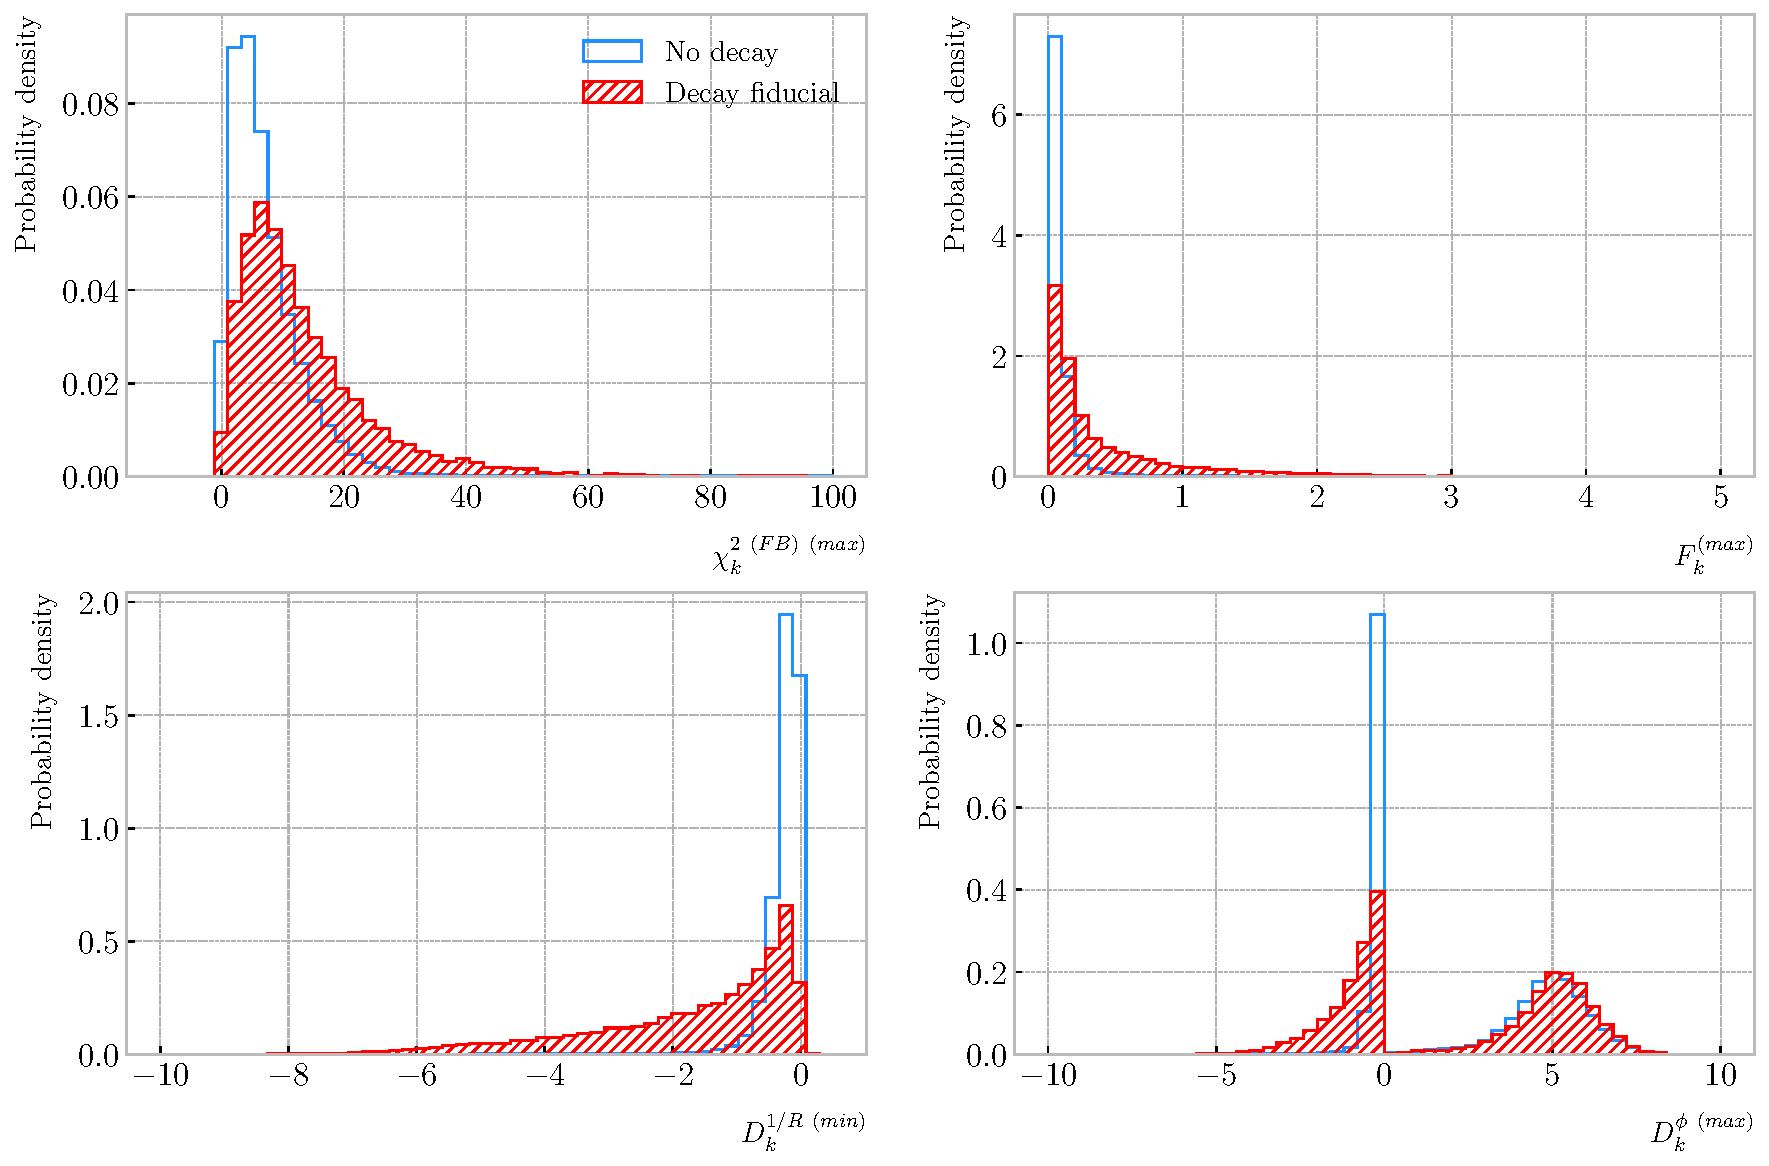
\includegraphics[width=.85\linewidth]{Images/GArSoft_PID/pion_decay/pion_decay_variables.pdf}
	\caption[Distributions of the extrema of $\chi^{2 \ (FB)}_{k}$, $F_{k}$, $D^{1/R}_{k}$, and $D^{\phi}_{k}$ for non-decaying and decaying reconstructed pion tracks.]{Distributions of the extrema of $\chi^{2 \ (FB)}_{k}$ (top left panel), $F_{k}$ (top right panel), $D^{1/R}_{k}$ (bottom left panel) and $D^{\phi}_{k}$ (bottom right panel) for non-decaying reconstructed pion tracks (blue) and tracks which include the decay inside the fiducial volume (red).}
	\label{fig:breakpoint_variables}
\end{figure}

Figure \ref{fig:breakpoint_variables} contains the distributions of the maxima of $\chi^{2 \ (FB)}_{k}$, $F_{k}$ and $D^{\phi}_{k}$ and the minima of $D^{1/R}_{k}$ for a sample of non-decaying pion tracks (blue) and another sample of reconstructed tracks containing part of the pion and the daughter muon from a decay inside the fiducial volume (red). Notice that, even though the values of $F^{(max)}_{k}$ for the decay sample are typically larger than for the non-decaying one, just a small fraction of the events go beyond the aforementioned value of $F=2.60$. Therefore, from a practical point of view, it is not the most efficient variable to use for selecting the decay events.

However, looking at the $D^{1/R \ (min)}_{k}$ distribution we can see there is a big difference between non-decaying and decaying events in this variable. One can use a combination of these four variables to distinguish between the pion decay events (signal) and the non-decaying pions (background).

\begin{figure}[t]
	\centering
	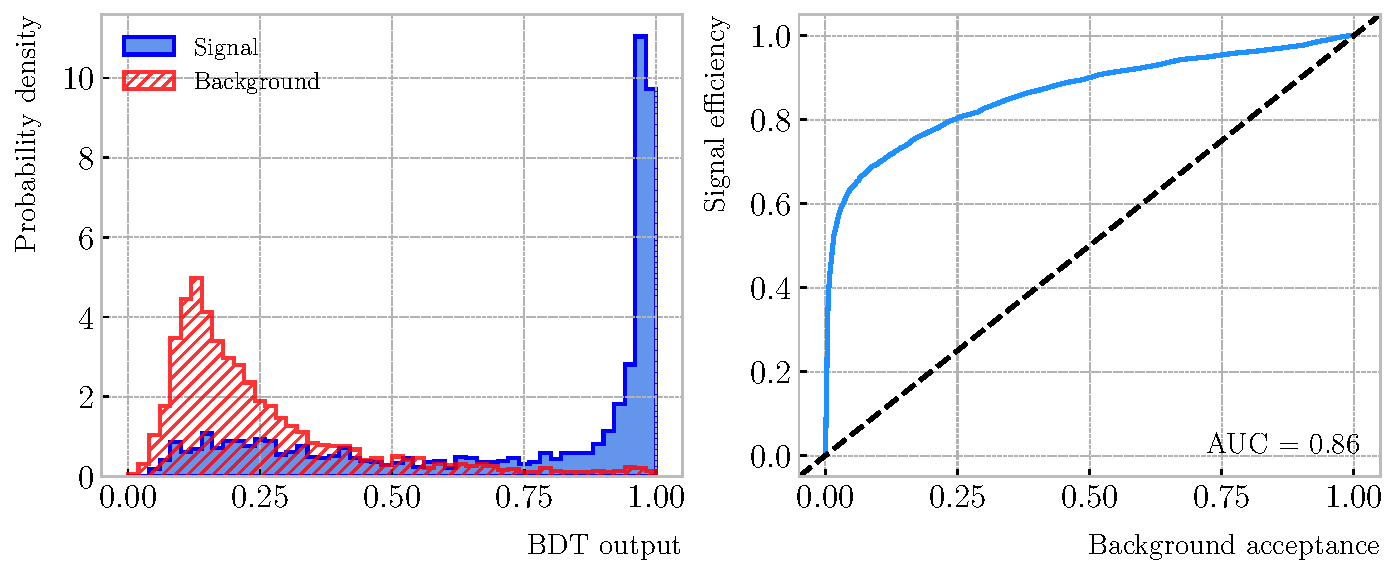
\includegraphics[width=.85\linewidth]{Images/GArSoft_PID/pion_decay/pion_decay_summary_bdt.pdf}
	\caption[Outputs of the \gls{bdt} classifier for a test sample of decaying pion+muon tracks and non-decaying pion tracks.]{Left panel: distributions of the predicted probabilities assigned by the \gls{bdt} classifier for a test sample of decaying pion+muon tracks (blue) and non-decaying pion tracks (red). Left: signal efficiency versus background acceptance (ROC curve) obtained from the \gls{bdt} for the test sample.}
	\label{fig:breakpoint_bdt}
\end{figure}

\begin{figure}[t]
	\centering
	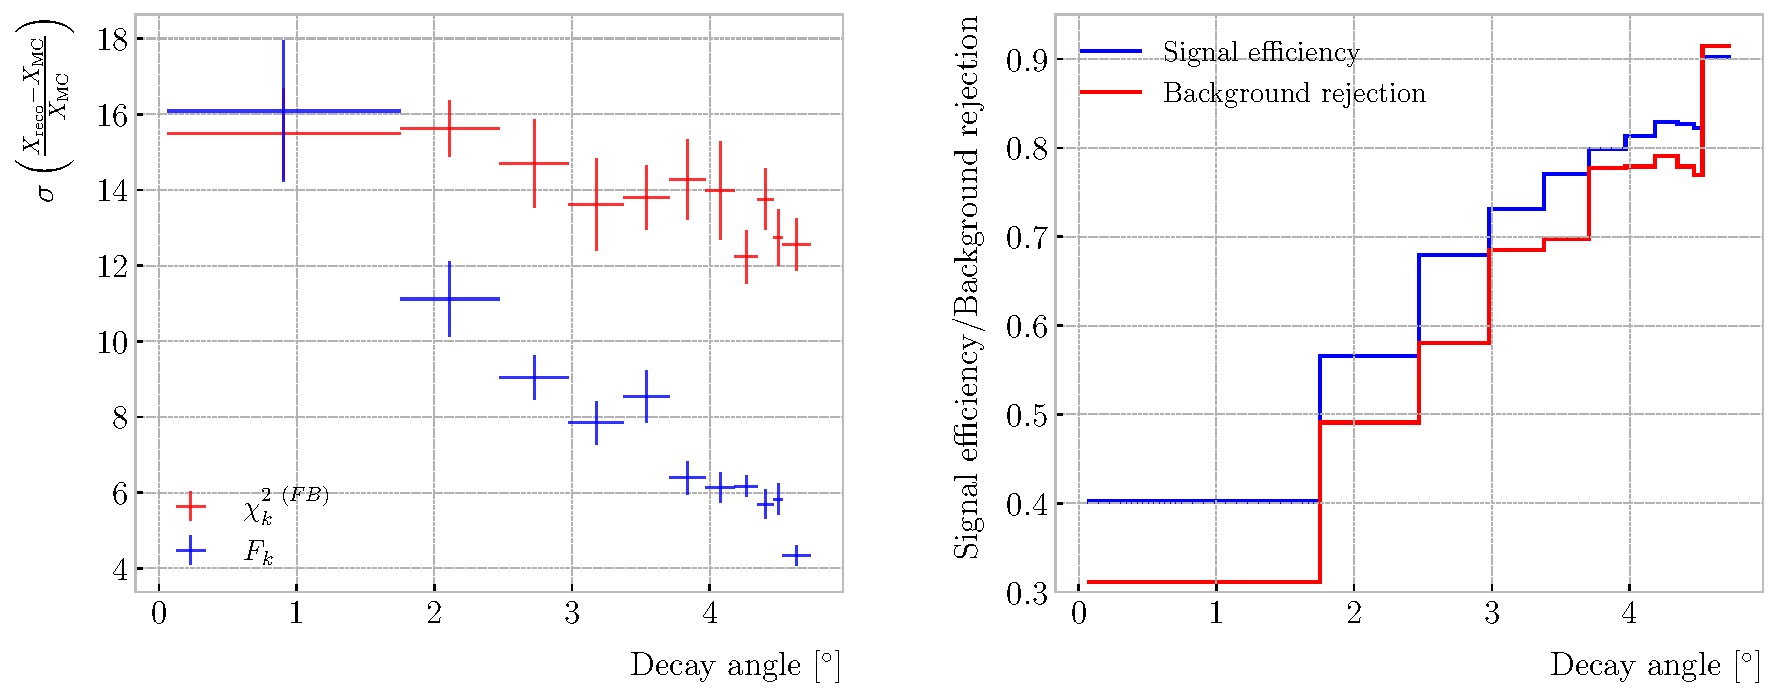
\includegraphics[width=.85\linewidth]{Images/GArSoft_PID/pion_decay/pion_decay_angle_summary2.pdf}
	\caption[Dependence of the decay position finding resolution and \gls{bdt} performance on the true value of the decay angle.]{Left panel: dependence of the decay position finding resolution on the true value of the decay angle for the $\chi_{k}^{2 \ (FB)}$ (red) and $F_{k}$ (blue) methods. Right panel: signal efficiency (blue line) and background rejection (red line) from the \gls{bdt} classifier versus true decay angle.}
	\label{fig:breakpoint_angle}
\end{figure}

An approach to this classification could be using a \gls{bdt}. Training a \gls{bdt} with $400$ estimators and a maximum depth of $4$ I can obtain an efficient classification without overtraining. Figure \ref{fig:breakpoint_bdt} (left panel) shows the distribution of probabilities predicted by the \gls{bdt} for a test sample. The signal efficiency as a function of background acceptance, the so-called ROC curve, is shown in Fig. \ref{fig:breakpoint_bdt} (right panel). With a relative importance of $0.83$, the most important variable turned out to be $D_{k}^{1/R \ (min)}$.

One thing we can check is how the resolution to the decay and the signal efficiency in the classification changes with the true decay angle. Using an equal-frequency binning for the decay angles, we can repeat the previous steps for each bin.

Figure \ref{fig:breakpoint_angle} (left panel) shows the dependence on the decay angle of the decay finding resolution. We can see that for the $\chi_{k}^{2 \ (FB)}$ maximum location method the resolution consistently lies between $12$ to $16\%$. However, the $F^{(max)}_{k}$ approach gives a significantly better resolution for high angle values, reaching the $4-6\%$ range for decay angles $\geq 4^{\circ}$.

For the classification dependence on the angle, I use the same classifier I trained before but evaluating the test sample for each individual angular bin. I compute the signal efficiency in each bin for a fixed value of the background rejection, in this case $90\%$. Similarly, for the background rejection estimation I use a fixed signal efficiency value of $90\%$. Figure \ref{fig:breakpoint_angle} (right panel) represents the change in signal efficiency (blue) and background rejection (red) with the value of the true decay angles.

\section{Neutral particle identification}
\label{section:neutral}

\subsection{ECal clustering}

Another important reconstruction item is the clustering algorithm of \gls{ecal} hits in GArSoft. The default module features a \gls{nn} algorithm that treats all hits in the same way, independently of the layer each hit comes from. However, the current \gls{ecal} design of \gls{ndgar} has two very different types of scintillator layers. The inner layers are made out of tiles, which provide excellent angular and timing resolutions. On the other hand, the outer layers are cross scintillator strips. That way, an algorithm that treats hits from both kinds of layers differently may be able to improve the current performance.

Inspired by the reconstruction of \gls{t2k}'s ND280 downstream \gls{ecal} \cite{T2KUK2013}, the idea was to put together a clustering module that first builds clusters for the different \gls{ecal} views (tiles, strips segmented in the $x$ direction and strips segmented in $y$ direction), and then tries to match them together to form the final clusters.

Working on a module-by-module basis, the algorithm separates the hits depending on the layer type they come from. Then, it performs a \gls{nn} clustering for the 3 sets of hits separately. For the tile hits it clusters together all the hits which are in nearest-neighbouring tiles and nearest-neighbouring layers. For strip hits it looks at nearest-neighbouring strips and next-to-nearest-neighbouring layers (as the layers with strips along the two directions are alternated). For strip clusters an additional cut in the direction along the strip length is needed.

After this first clustering I then apply a recursive re-clustering for each collection of strip clusters based on a PCA method. In each case, the algorithm loops over the clusters with $N_{hits}\geq2$, computing the centre of mass and three principal components. Propagating these axes up to the layers of the rest of the clusters, we check if the propagated point and the centre of mass of the second cluster are within next-to-nearest-neighbouring strips. An additional cut in the direction along the strip length is also needed. Moreover, I require that the two closest hits across the two clusters are at most in next-to-nearest-neighbouring strips. I merge the clusters if these three conditions are satisfied. The re-clustering is repeated until no more cluster pairs pass the cuts.

The clusters in each strip view are combined if their centres of mass are close enough and they point in the same direction. An alternative approach for the strip cluster merging could be to compute the overlap between the ellipsoids defined by the principal axes of the clusters, and then merge the pair if the overlap exceeds some threshold. Further study is needed to understand if this change would have an impact in the overall clustering performance.

To merge the tile clusters to the combined strip clusters, I propagate the principal axis of the strip cluster towards the inner layers, up to the centre of mass layer of the tile cluster. I merge the clusters if the distance between the propagated point and the centre of mass is bellow a certain cut.

The last step is to check if clusters in neighbouring modules should be merged together, both across two barrel modules, across end cap modules and between barrel end cap modules. I check the distance between the two closest hits in the pair of clusters and merge them if it passes this and an additional directional cut.

\begin{comment}
	Figure \ref{fig:clustering_example} presents an example of the clustering steps relevant for strip layer hits, from the input hits (top left panel) to the \gls{nn} clustering (top right panel) and re-clustering (bottom left panel) for each strip view and the final merging strip clusters (bottom right panel). It shows the hits from a single \gls{ecal} barrel module in a $\nu_{\mu}$ \gls{cc} interaction event with a neutral pion and a proton in the final state. The two clusters on the left correspond to the photon pair from the $\pi^{0}$ decay and the one on the upper right corner is associated to the proton.
\end{comment}

\begin{figure}[t]
	\centering
	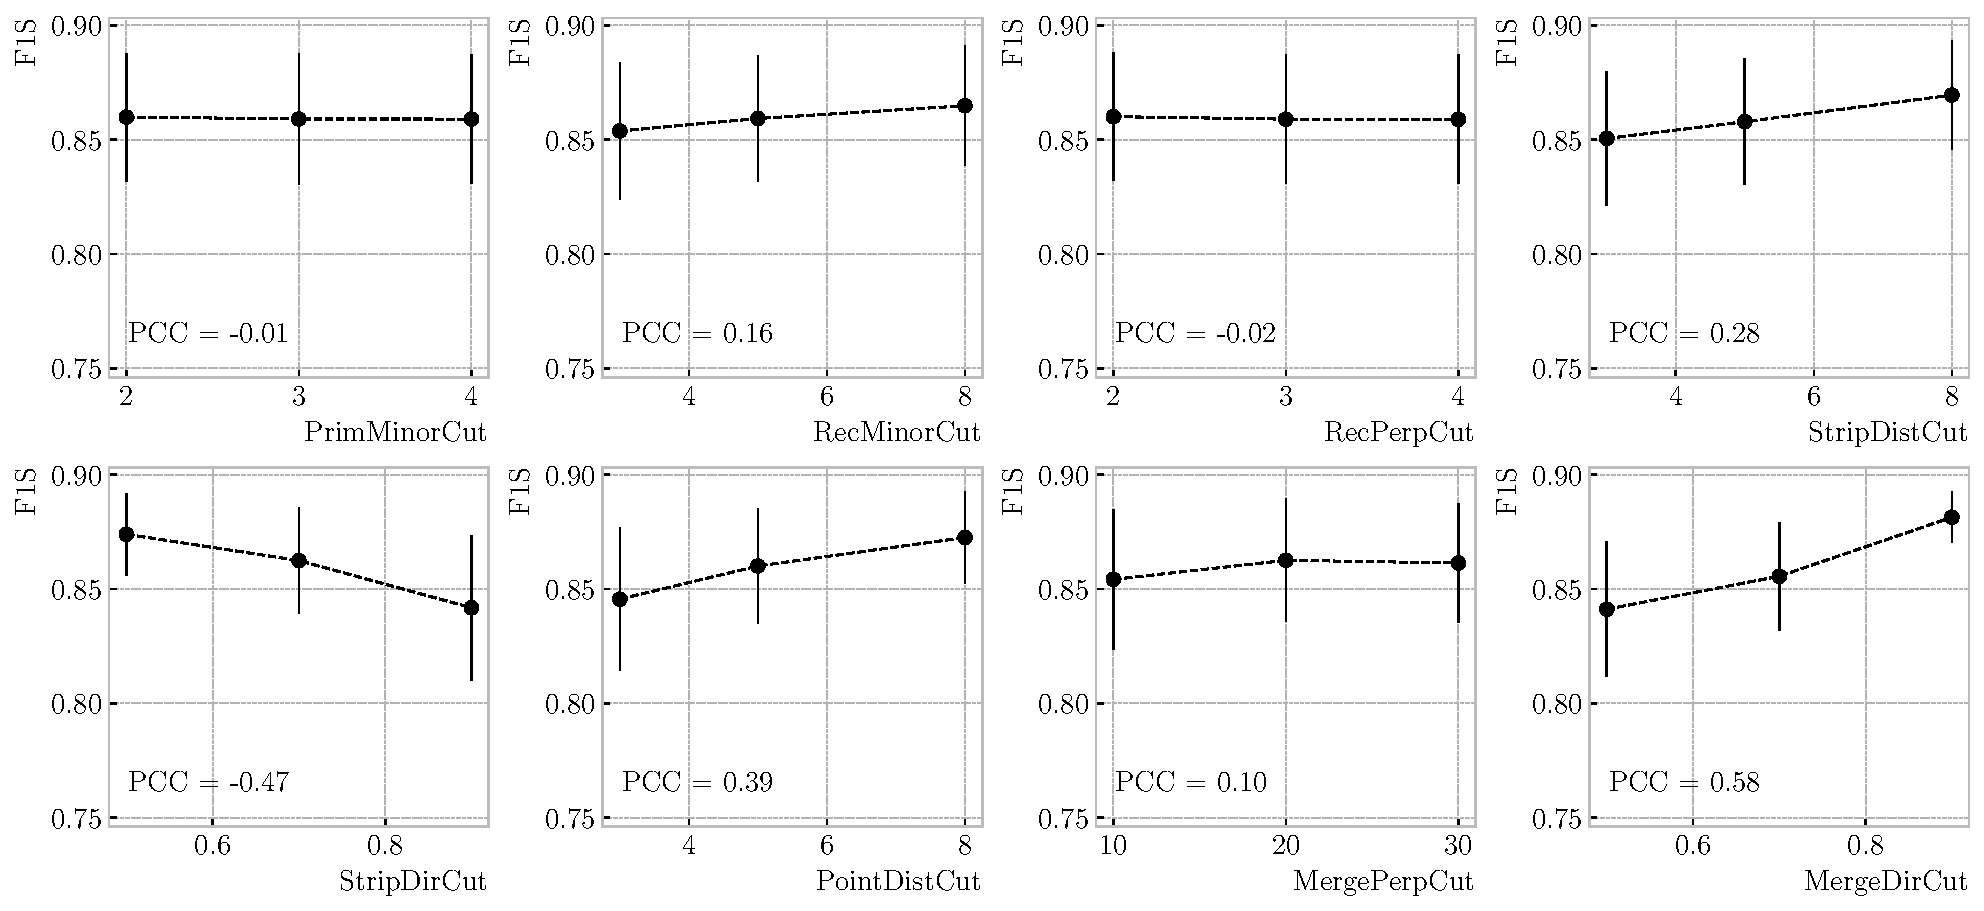
\includegraphics[width=.99\linewidth]{Images/GArSoft_PID/Neutral/coolcluster_optimisation_F1S.pdf}
	\caption[Mean values of the $F_{1}$-score marginal distributions for the different free parameters of the new clustering algorithm.]{Mean values of the $F_{1}$-score marginal distributions for the different free parameters of the new clustering algorithm, with the error bars representing one standard deviation around the mean. The $F_{1}$-score values were computed for the 6561 possible parameter configurations using 1000 $\nu_{\mu}$ \gls{cc} interaction events.}
	\label{fig:clustering_optimisation}
\end{figure}

\begin{table}[t]
	\caption{Summary of parameters and sampled values used in the optimisation of the clustering algorithm.}
	\begin{center}
		\begin{small}
			\begin{tabular}{l|l|l|p{7cm}}
				Name         & Units  & Sampled values & Description                                                                  \\[2mm] \hline
				\rule{0pt}{1.1\normalbaselineskip}PrimMinorCut & strips & 2, 3, 4        & Distance along strip length in \gls{nn} clustering                                 \\[3mm]
				RecMinorCut  & strips & 3, 5, 8        & Distance between propagated point and CM along strip length in re-clustering \\[8mm]
				RecPerpCut   & strips & 2, 3, 4        & Closest hit pair distance in re-clustering                                   \\[3mm]
				StripDistCut & strips & 3, 5, 8        & Distance between CMs in strip cluster merging                                \\[3mm]
				StripDirCut  & cos    & 0.5, 0.7, 0.9  & Main axes direction cut in strip cluster merging                             \\[3mm]
				PointDistCut & tiles  & 3, 5, 8        & Distance between propagated point and CM in strip-tile matching              \\[8mm]
				MergePerpCut & cm     & 10, 20, 30     & Closest hit pair distance in module merging                                  \\[3mm]
				MergeDirCut  & cos    & 0.5, 0.7, 0.9  & Main axes direction cut in module merging                                   
			\end{tabular}
		\end{small}
	\end{center}
	\label{tab:clustering_optimisation}
\end{table}

This algorithm has a total number of eight free parameters that need to be optimised. I used a sample of 1000 $\nu_{\mu}$ \gls{cc} interactions in order to obtain the optimal configuration of clustering parameters. This sample was generated up to the default \gls{ecal} hit clustering level, so then I could run the new clustering algorithm each time with a different configuration of parameters. As the number of parameters is relatively large, I only performed a coarse-grained scan of the parameter space. Sampling each of the eight parameters at three different points each I obtain 6561 different configurations. These parameters, together with the used values, are summarised in Tab. \ref{tab:clustering_optimisation}.

In order to measure the performance of the clustering, I use a binary classification approach. For each formed cluster, I identify the \texttt{Geant4} Track ID of the matching \gls{mc} particle and the energy fraction of each hit. Then, I assign to each cluster the Track ID with the highest total energy fraction. For each of the different Track IDs associated to the clusters, I select the cluster with the highest energy (only from the hits with the same Track ID). I identify such a cluster as the main cluster for that Track ID. I count as true positives (TPs) the hits with the correct Track ID in each main cluster. False positives (FPs) are the hits with the incorrect Track ID for the cluster they are in, not only main clusters. The false negatives (FNs) are the hits with the correct Track ID in clusters other than the main.

Figure \ref{fig:clustering_optimisation} shows the computed $F_{1}$-score values for the different cuts. In each case, the central value represents the mean of the $F_{1}$-score distribution for the specified value of the corresponding variable, and the vertical error bar represents one standard deviation around the mean. Also shown are the Pearson correlation coefficients of these central values. We can see that five of the variables have a sizeable effect on the $F_{1}$-score, with an absolute difference between the last and first values as big as $4\%$.

The working configuration is obtained as follows. I first select all configurations with purity $\geq90\%$. Among those, I choose the combinations that yield the maximum $F_{1}$-score. If more than one configuration remains, I select the one with the highest sensitivity. Doing so, I end up with a parameter configuration with an efficiency of $88\%$ and a $90\%$ purity. Compared with the default algorithm, which gives an efficiency of $76\%$ and a purity of $91\%$ for the same sample, I have managed to improve the efficiency by a factor of $1.16$.

\subsection[\texorpdfstring{$\pi^{0}$}{pi0} reconstruction]{\boldmath\texorpdfstring{$\pi^{0}$}{pi0} reconstruction}

\begin{figure}[t]
	\begin{subfigure}{0.5\textwidth}
		\centering
		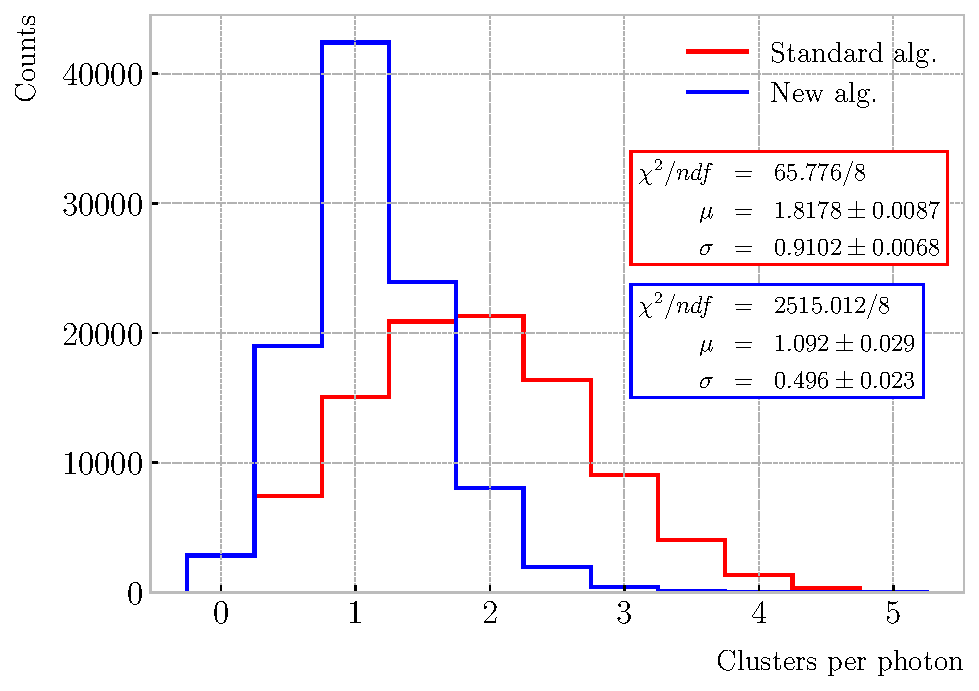
\includegraphics[width=.99\linewidth]{Images/GArSoft_PID/Neutral/coolcluster_clusters_per_photon.pdf}
	\end{subfigure}
	\begin{subfigure}{0.5\textwidth}
		\centering
		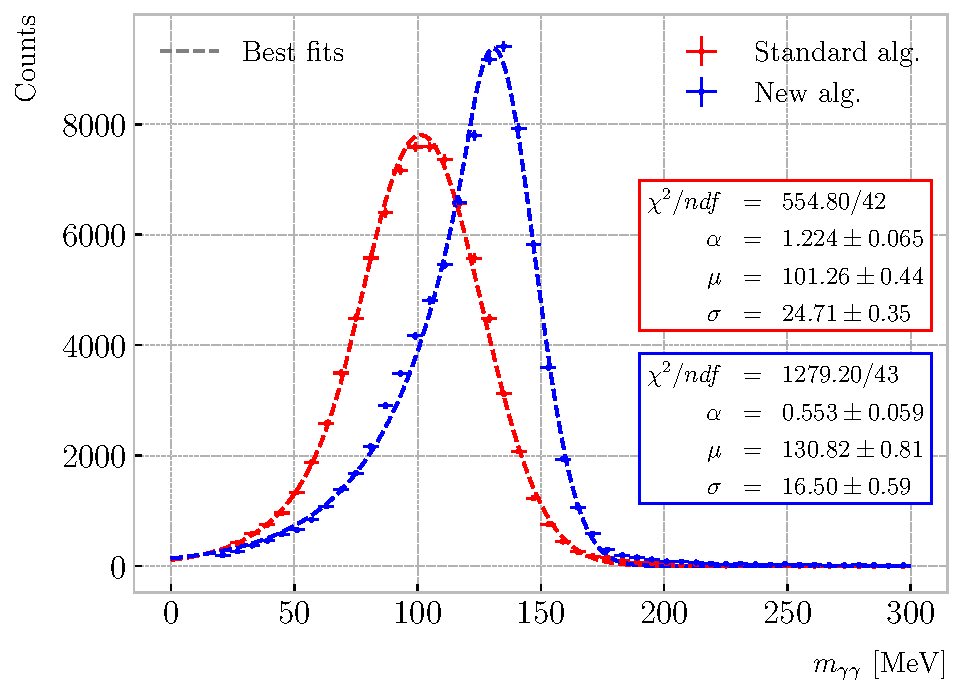
\includegraphics[width=.99\linewidth]{Images/GArSoft_PID/Neutral/coolcluster_invariant_mass_vertex.pdf}
	\end{subfigure}
	\caption[Number of cluster per photon and invariant mass distributions for photon pairs from single $\pi^{0}$ events using the standard and new \gls{ecal} clustering algorithms.]{Left panel: distributions of the number of \gls{ecal} clusters per photon from $\pi^{0}$ decays for the standard (red) and new (blue) clustering algorithms. Right panel: reconstructed invariant mass distributions for photon pairs from single $\pi^{0}$ events using the standard (red) and new (blue) \gls{ecal} clustering algorithms.}
	\label{fig:clustering_pizero}
\end{figure}

One of the potential applications of the new \gls{ecal} hit clustering is the reconstruction of neutral particles, in particular pions. Neutral pions decay promptly after being produced, through the $\pi^{0} \rightarrow \gamma\gamma$ channel $(98.823 \pm 0.034)\%$ of the time \cite{ParticleDataGroup2024}. The photon pair does not leave any traces in the \gls{hpgtpc} (unless one or both of them converts into an electron-positron pair), but each of them will produced an electromagnetic shower in the \gls{ecal}.

To test the potential impact of the new algorithm on the $\pi^{0}$ reconstruction, I generated a \gls{mc} sample of single, isotropic neutral pions inside the \gls{hpgtpc}. All pions were generated with a momentum of $500 ~ \mathrm{MeV}/c$, and their initial positions were uniformly sampled inside a $2 \times 2 \times 2 \ \mathrm{m}$ box aligned with the centre of the \gls{hpgtpc}. I ran both the default and the new clustering algorithms, using for the latter the optimised configuration discussed above.

The first thing to notice is that the number of clusters produced per photon has decreased. Figure \ref{fig:clustering_pizero} (left panel) shows these distributions for the default (red) and new (blue) algorithms. Using a simple Gaussian fit, we see that the mean number of \gls{ecal} clusters per photon went from $1.82 \pm 0.01$ to $1.09 \pm 0.03$. This effectively means that with the new algorithm the \gls{ecal} activity of one true particle is typically reconstructed as a single object. From the reconstruction point of view this can be an advantage. As now most of the photon energy ends up in a single \gls{ecal} cluster, I can simply use cluster pairs to identify the $\pi^{0}$ decay.

In general, one calculates the invariant mass of the photon pair as:
\begin{equation}
	m_{\gamma\gamma} = \sqrt{2E_{1}E_{2}(1-\mathrm{cos} \ \theta)},
\end{equation}
where $E_{i}$ are the energies of the photons and $\theta$ the opening angle between them. In this case, I can use the energies deposited in the \gls{ecal} and their incident directions. This quantity is computed for all possible pairs of clusters, using their position together with the true decay point. In a more realistic scenario, e.g. $\nu_{\mu}$ \gls{cc} interaction, one could use the position of the reconstructed primary vertex instead. I also tried to use the principal direction of the clusters, but that approach gave considerably worse results. For each event, I only keep the pair with the invariant mass closest to the true $\pi^{0}$ mass value.

Figure \ref{fig:clustering_pizero} (right panel) shows the invariant mass distributions for the photon pairs I get using the default (red) and the new (blue) \gls{ecal} clustering algorithms. For the fit I use a modified version of the Crystal Ball function \cite{Gaiser1982}, obtained by taking the limit where the parameter controlling the power-law tail goes to infinity:
\begin{equation}
	f(x; N, \mu, \sigma, \alpha) = N \cdot
	\left\{
	\begin{array}{ll}
		\mathrm{e}^{\frac{\alpha(2x-2\mu+\alpha\sigma)}{2\sigma}};& x \leq \mu - \alpha\sigma,\\
		\mathrm{e}^{-\frac{(x-\mu)^{2}}{2\sigma^{2}}};& x > \mu - \alpha\sigma.
	\end{array}
	\right.
\end{equation}
Comparing the fitted mean and standard deviation values for the Gaussian cores, we see that the distribution for the new algorithm is a $67\%$ narrower and also peaks much closer to the true $m_{\pi^{0}}$ value, going from $101.3 \pm 0.4 \ \mathrm{MeV}$ to $130.8 \pm 0.6 \ \mathrm{MeV}$.